\documentclass{beamer}
\usepackage[utf8]{inputenc}

\usepackage[final]{pdfpages}

\usepackage{fourier} %font utopia imported
\usepackage{tabularx}
\usepackage{multirow}
\usepackage{booktabs}
\usepackage{stackengine}
\usepackage{xcolor}

\usefonttheme{serif}
\usetheme{Madrid}
\usecolortheme{beaver}
\newcommand{\etal}{\textit{et al.}}

\definecolor{good}{RGB}{81,135,35}
\definecolor{bad}{RGB}{142,42,42}

%------------------------------------------------------------
%This block of code defines the information to appear in the
%Title page
\title[] %optional
{Neural Networks based Speed-Torque Estimators for Induction Motors and Performance Metrics}


\author[Verma \etal] % (optional)
{S.~Verma\inst{1,2} \and N.~Henwood\inst{2} \and M.~Castella\inst{3} \and A.~K.~Jebai\inst{2} \and J.C.~Pesquet\inst{1}}

\institute[CVN and STIE] % (optional)
{
  \inst{1}%
  Universit\'{e} Paris-Saclay, CentraleSup\'{e}lec, Inria, Centre de Vision Num\'{e}rique
  \and
  \inst{2}%
  Schneider Toshiba Inverter Europe
  \and
  \inst{3}%
  SAMOVAR, T\'{e}l\'{e}com SudParis, Institut Polytechnique de Paris
}

\date[IECON 2020] % (optional)
{46th Annual Conference of the IEEE Industrial Electronics Society}

\logo{

\includegraphics[height=0.7cm]{images/supelec.png}

\includegraphics[height=0.7cm]{images/se.png}

\includegraphics[height=0.7cm]{images/tsp.png}}

%End of title page configuration block
%------------------------------------------------------------
% \begin{titlepage}
% \includepdf[pages=-,pagecommand={},width=\textwidth]{auth.pdf}
% \end{titlepage}


%------------------------------------------------------------
%The next block of commands puts the table of contents at the
%beginning of each section and highlights the current section:

\AtBeginSection[]
{
  \begin{frame}
    \frametitle{Table of Contents}
    \tableofcontents[currentsection]
  \end{frame}
}
%------------------------------------------------------------


\begin{document}

%The next statement creates the title page.
\frame{\titlepage}


%---------------------------------------------------------
%This block of code is for the table of contents after
%the title page
\begin{frame}
\frametitle{Table of Contents}
\tableofcontents
\end{frame}
%---------------------------------------------------------


\section{Introduction}

%---------------------------------------------------------
%Changing visivility of the text
\begin{frame}
\frametitle{Introduction}
Evaluating neural networks (NNs) used in induction motor use case using performance metrics.

\begin{itemize}
    \item Physics for dynamics modeling.
    \item ML methods for control and fault detection.
    \item Large industrial sensor datasets.
    \item Performance metrics to evaluate NN.
\end{itemize}
\end{frame}

%---------------------------------------------------------


%---------------------------------------------------------
%Example of the \pause command
\begin{frame}
\frametitle{Problem Statement}

\textit{Estimating speed and torque from current and voltage of an induction motor using NNs.}

\begin{figure}[ht!]
    \centering
    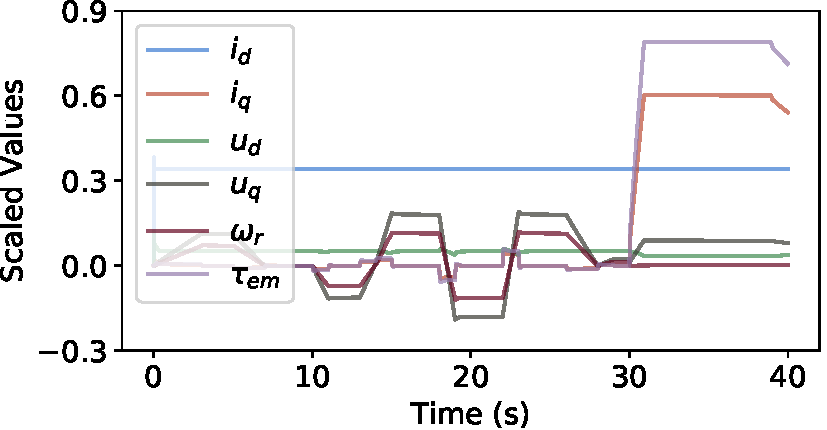
\includegraphics[scale=0.4]{images/sim.pdf}
    \caption{First 40 seconds of a simulated electrical motor operation.}
    \label{fig:sim_raw_data}
\end{figure}

\end{frame}
%---------------------------------------------------------

%---------------------------------------------------------
%Highlighting text
% \begin{frame}
% \frametitle{Contributions}

% \begin{itemize}
%     \item We use data driven approach to model dynamics by learning input-output relationship.
%     \item We evaluate 8 neural networks methods.
%     \item We show how performance metrics overcome certain limitations of standard machine learning metrics.
%     \item We introduce first and largest dataset of simulated and real world motor.
%     \item We release our code and dataset. Available here https://sagarverma.github.io/dynamics.html
% \end{itemize}

% \end{frame}
%---------------------------------------------------------




\section{Related Work}

%---------------------------------------------------------
%Highlighting text
\begin{frame}
\frametitle{Physical Modeling}

Model based controller requires modeling dynamics.
\begin{itemize}
    \item Controller design with known parameters [\textit{Nicklasson \etal, 1997}].
    \item Controller design with uncertain parameters [\textit{Marino \etal, 1999}].
    \item State-space model of induction motor [\textit{Jadot \etal, 2009}].
    \item Analytical mechanics and energy consumption [\textit{Jebai \etal, 2014}].
\end{itemize}

\end{frame}
%---------------------------------------------------------

%---------------------------------------------------------
%Highlighting text
\begin{frame}
\frametitle{Neural Network based Modeling}

Control and fault detection using NNs.
\begin{itemize}
    \item NN fault classifiers [\textit{Silva \etal, 2013}].
    \item Currents and flux linkages coupling using RBF [\textit{Ortombina \etal, 2018}].
    \item Encoder-decoder learning input-output relationship [\textit{Verma \etal, 2020}].
\end{itemize}

\end{frame}
%---------------------------------------------------------


\section{Proposed Method}

%---------------------------------------------------------
%Highlighting text
\begin{frame}
\frametitle{Reference Trajectory Generator}

\begin{itemize}
    \item Generate reference speed and torque load
    \item Real world operating scenarios
    \item Conditional Hidden Markov model
    \item Paramtereized operating conditions
\end{itemize}

\end{frame}
%---------------------------------------------------------

%---------------------------------------------------------
%Highlighting text
\begin{frame}
\frametitle{Reference Trajectory Generator}

\begin{figure}[ht!]
    \centering
        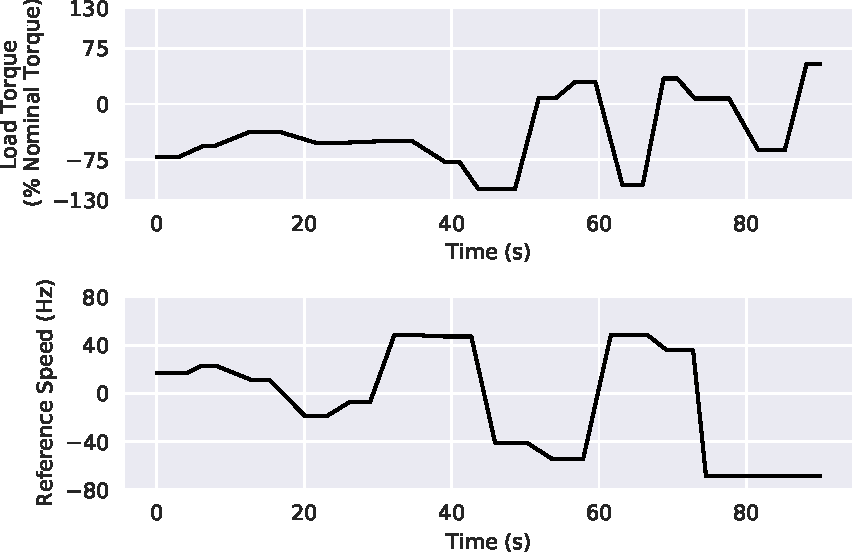
\includegraphics[scale=0.5]{images/train.pdf}
    \caption{Generated reference speed and load torque trajectories.}
    \label{fig:random}
    \vspace{-1em}
\end{figure}

\end{frame}
%---------------------------------------------------------

%---------------------------------------------------------
%Highlighting text
\begin{frame}
\frametitle{Nonlinear State-Space Motor Model}

\begin{itemize}
    \item Generate simulation data.
    \item Fifth-order nonlinear state space model [\textit{Jadot \etal, 2009}]
    \item Widely used in industrial paradigm.
    \item Explained in \textbf{Physical Modeling: A}.
\end{itemize}

\end{frame}

%---------------------------------------------------------
%Highlighting text
% \begin{frame}
% \frametitle{Nonlinear State-Space Motor Model}

% \begin{figure}[ht!]
%     \centering
%         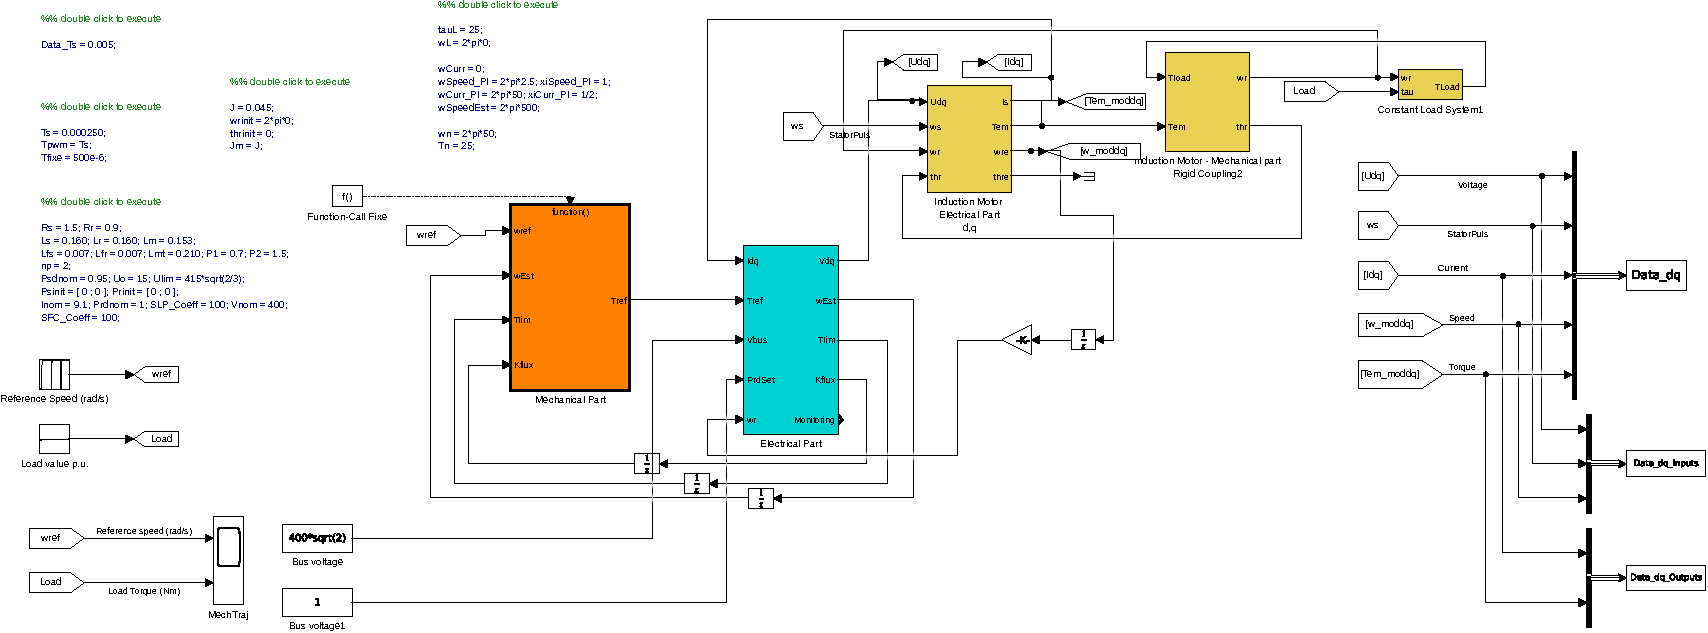
\includegraphics[scale=0.4]{images/fvc.pdf}
%     \caption{Nonlinear state-space model in Simulink.}
%     \label{fig:random}
%     \vspace{-1em}
% \end{figure}

% \end{frame}
%---------------------------------------------------------

%---------------------------------------------------------
%Highlighting text
\begin{frame}
\frametitle{Standard Neural Networks}

Three standard networks from [\textit{Verma \etal, 2020}]

\begin{itemize}
    \item Four layer Fully Connected Network (\textbf{FCN})
    \item Two layer Long-Short Term Memory Network (\textbf{LSTM})
    \item Four layer Convolutional Neural Network (\textbf{CNN})
\end{itemize}


\end{frame}
%---------------------------------------------------------

%---------------------------------------------------------
%Highlighting text
\begin{frame}
\frametitle{Four layer Fully Connected Network (FCN)}

\begin{figure}[ht!]
    \centering
        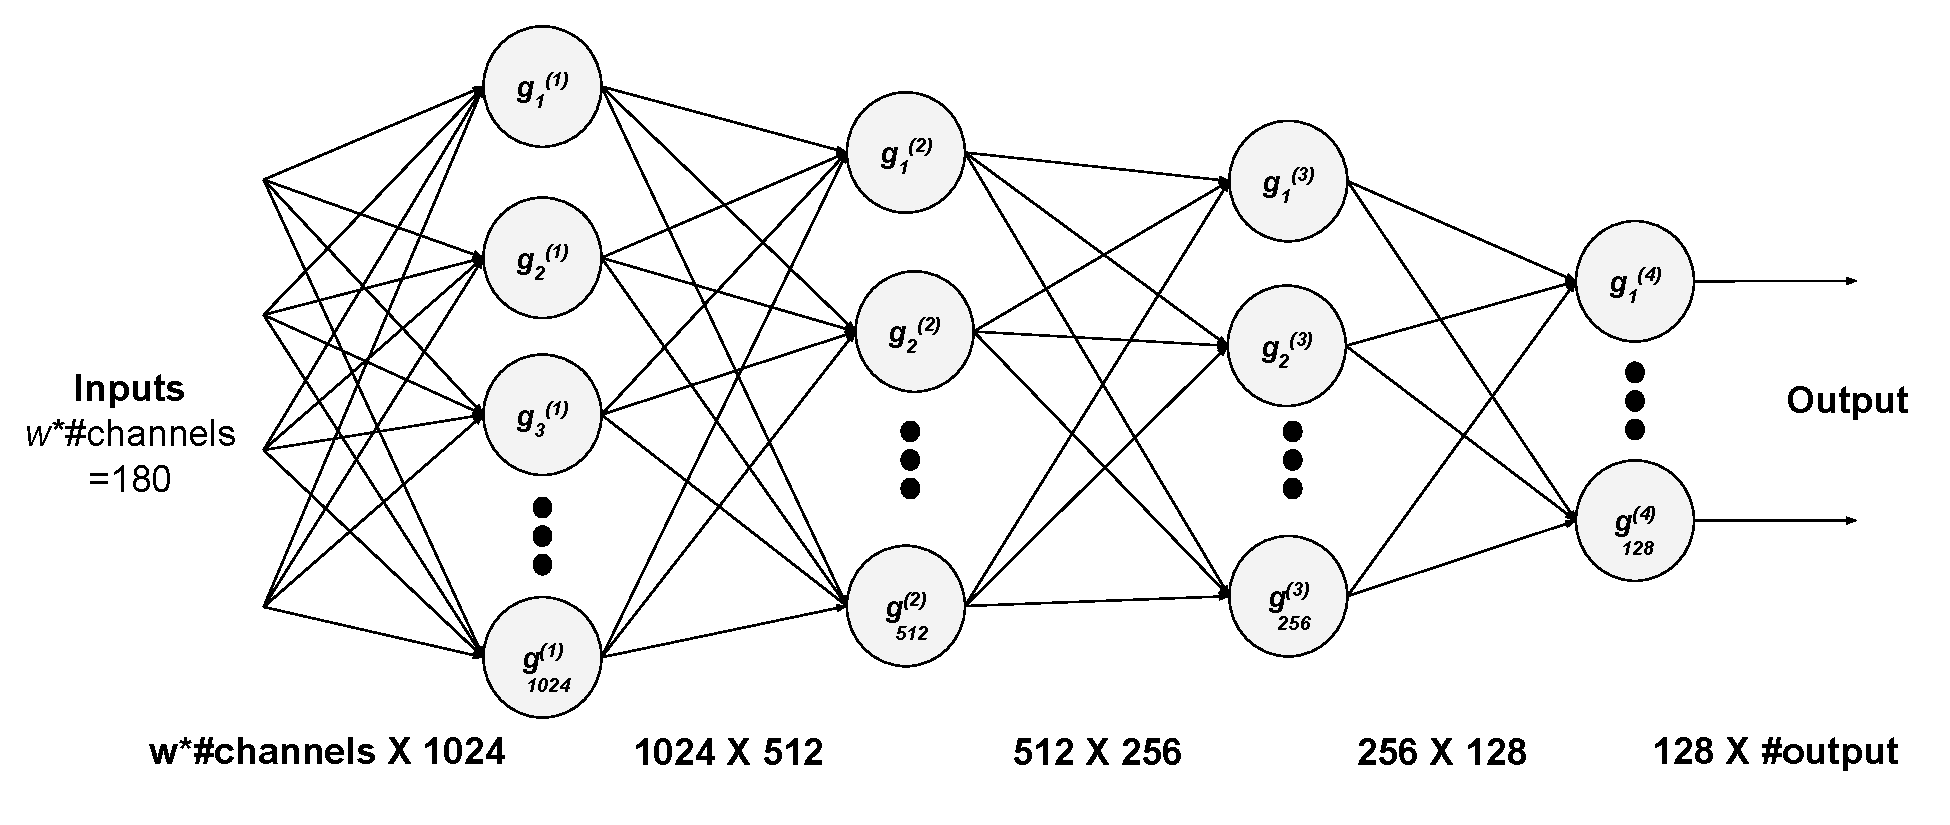
\includegraphics[scale=0.3]{images/ffn.pdf}
    \caption{Fully Connected Network.}
    \label{fig:random}
    \vspace{-1em}
\end{figure}

\end{frame}
%---------------------------------------------------------

%---------------------------------------------------------
%Highlighting text
\begin{frame}
\frametitle{Two layer Long-Short Term Memory Network (LSTM)}

\begin{figure}[ht!]
    \centering
        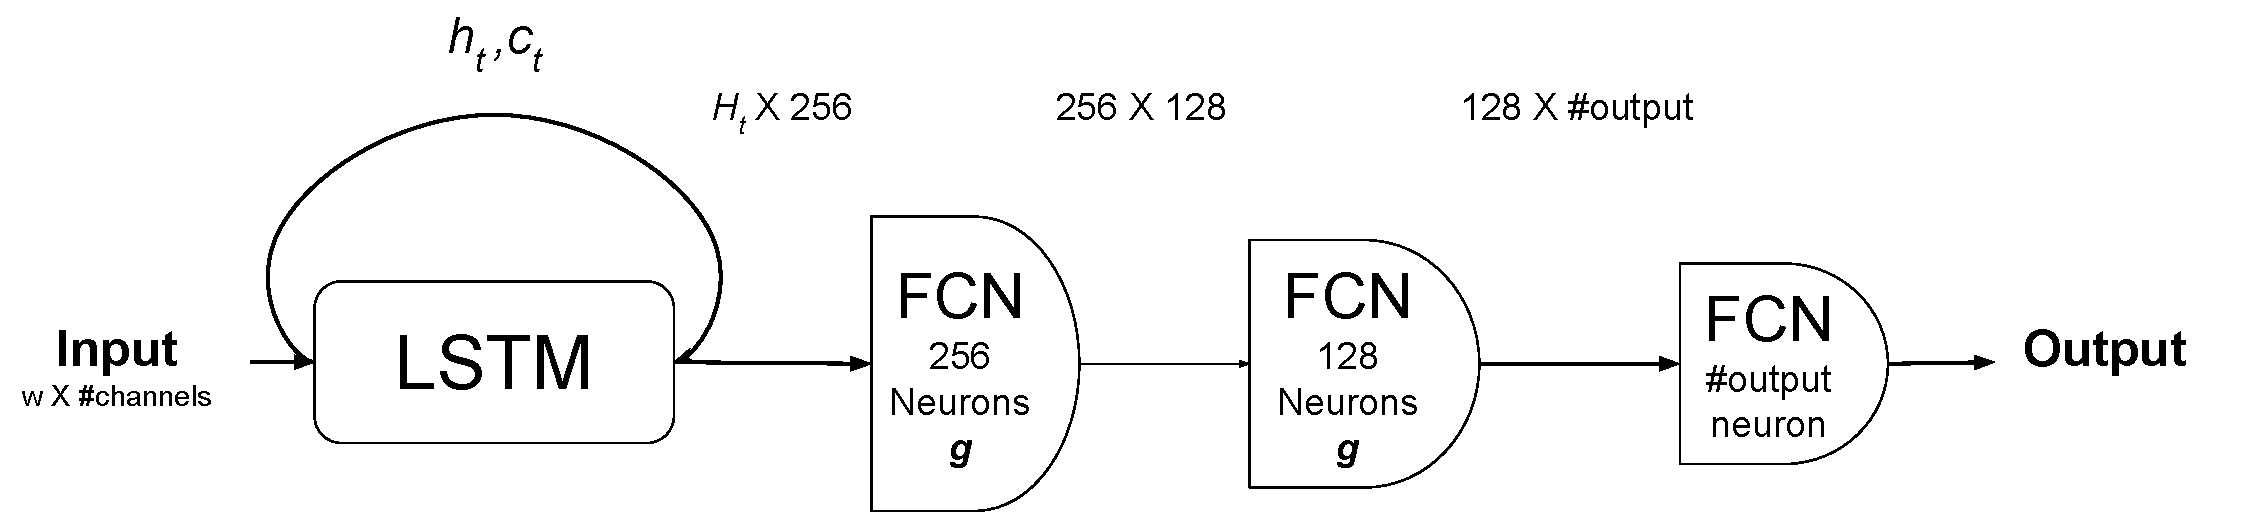
\includegraphics[scale=0.3]{images/lstm.pdf}
    \caption{Long-Short Term Memory Network.}
    \label{fig:random}
    \vspace{-1em}
\end{figure}


\end{frame}
%---------------------------------------------------------

%---------------------------------------------------------
%Highlighting text
\begin{frame}
\frametitle{Four layer Convolutional Neural Network (CNN)}

\begin{figure}[ht!]
    \centering
        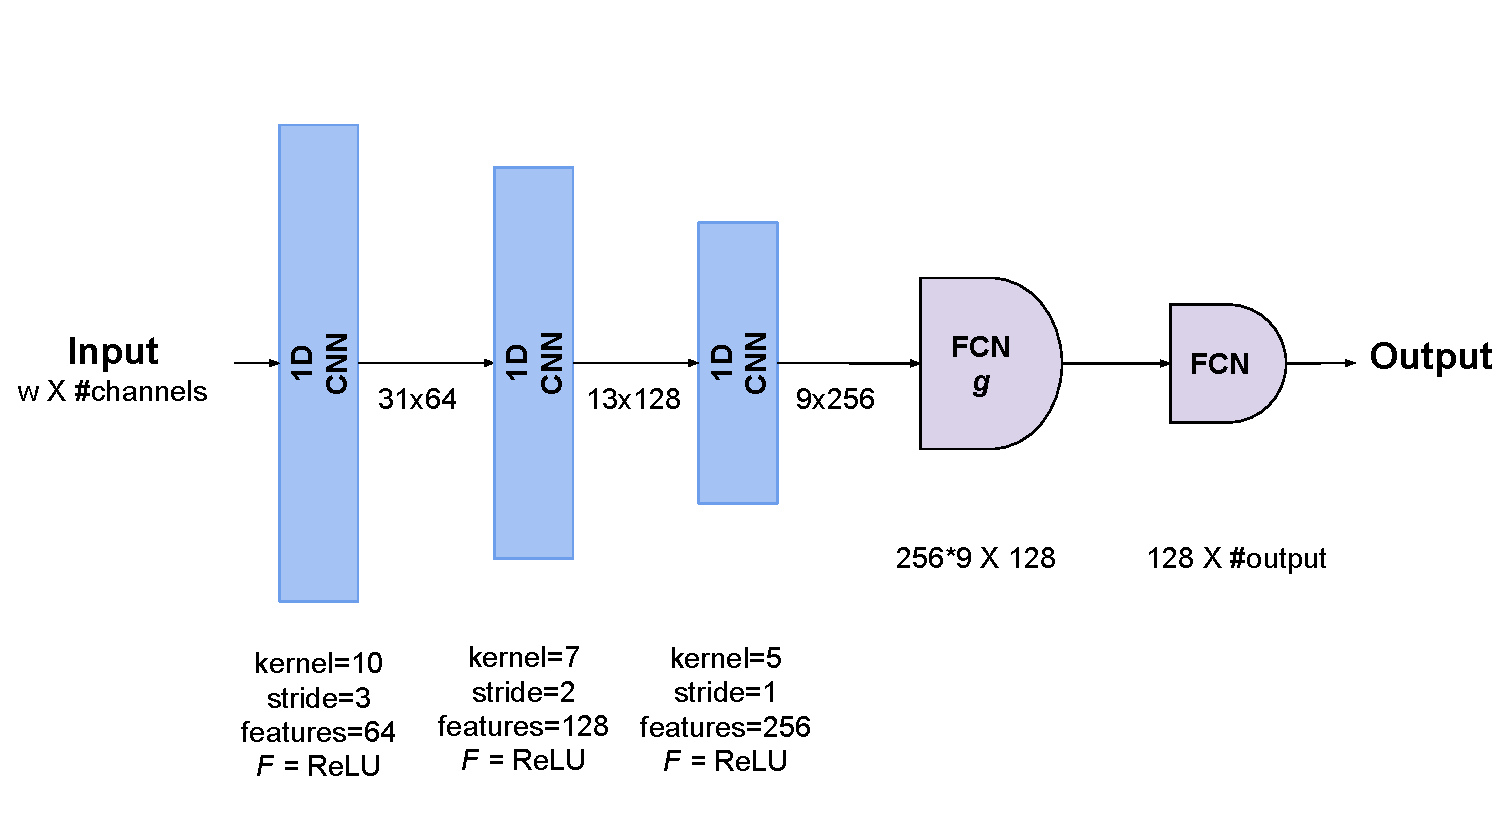
\includegraphics[scale=0.36]{images/cnn.pdf}
    \caption{Convolutional Neural Network.}
    \label{fig:random}
    \vspace{-1em}
\end{figure}


\end{frame}
%---------------------------------------------------------


%---------------------------------------------------------
%Highlighting text
\begin{frame}
\frametitle{Encoder-Decoder Networks}

Proven performance gain in temporal signal modeling.
\begin{itemize}
    \item Vanilla Encoder-Decoder (\textbf{Vanilla})
    \item Encoder-Decoder with Skip Connections (\textbf{Skip})
    \item Encoder-Decoder with Recurrent Skip Connections (\textbf{RNN})
    \item Encoder-Decoder with Bidirectional Recurrent Skip Connections (\textbf{BiRNN})
    \item Encoder-Decoder with Bidirectional Diaganolized Recurrent Skip Connections (\textbf{DiagBiRNN})
\end{itemize}
\end{frame}
%---------------------------------------------------------
%---------------------------------------------------------
%Highlighting text
\begin{frame}
\frametitle{Vanilla Encoder-Decoder (Vanilla)}

\begin{figure}[ht!]
    \centering
        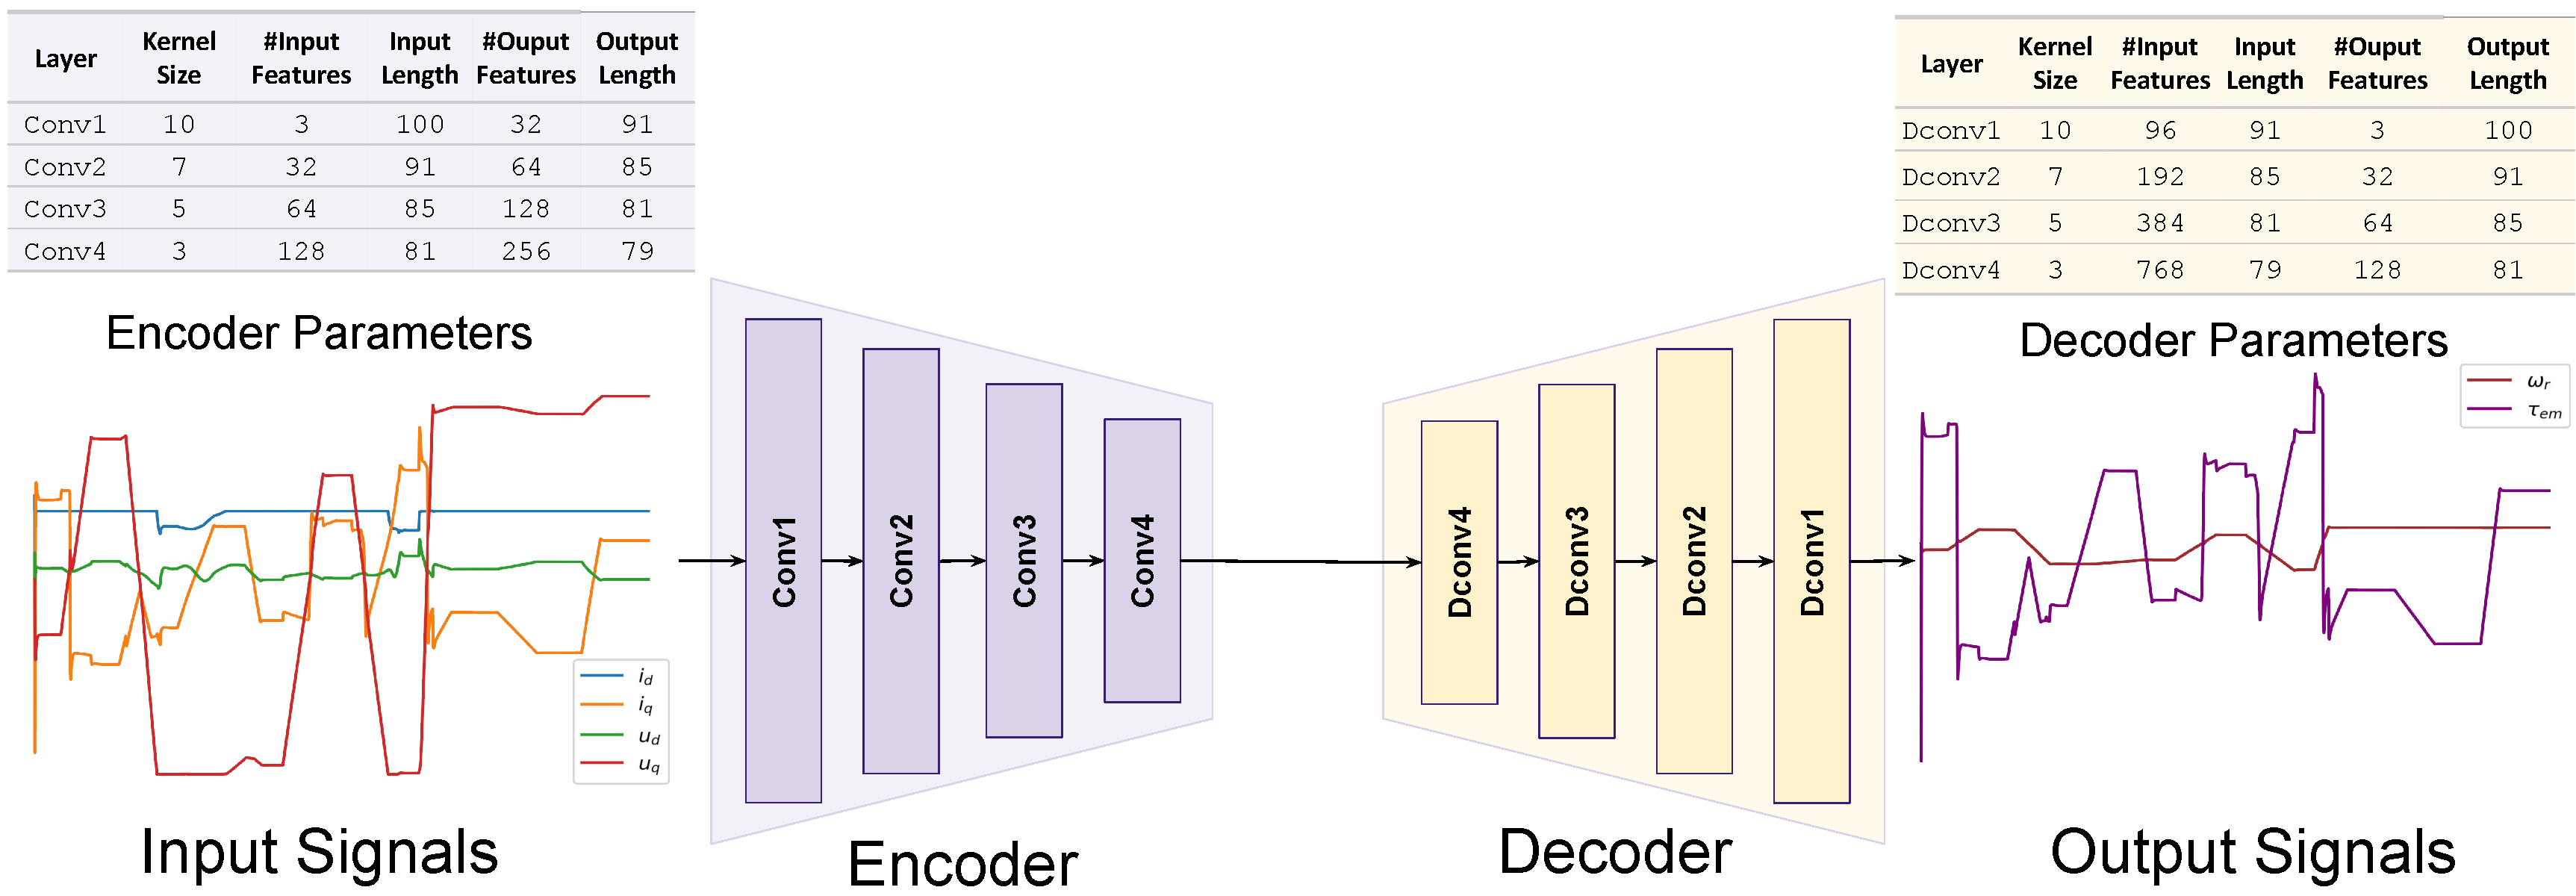
\includegraphics[scale=0.19]{images/ed_st.pdf}
    \caption{Vanilla}
    \label{fig:random}
    \vspace{-1em}
\end{figure}

\end{frame}


%---------------------------------------------------------
%Highlighting text
\begin{frame}
\frametitle{Encoder-Decoder with Skip Connections (Skip)}

\begin{figure}[ht!]
    \centering
        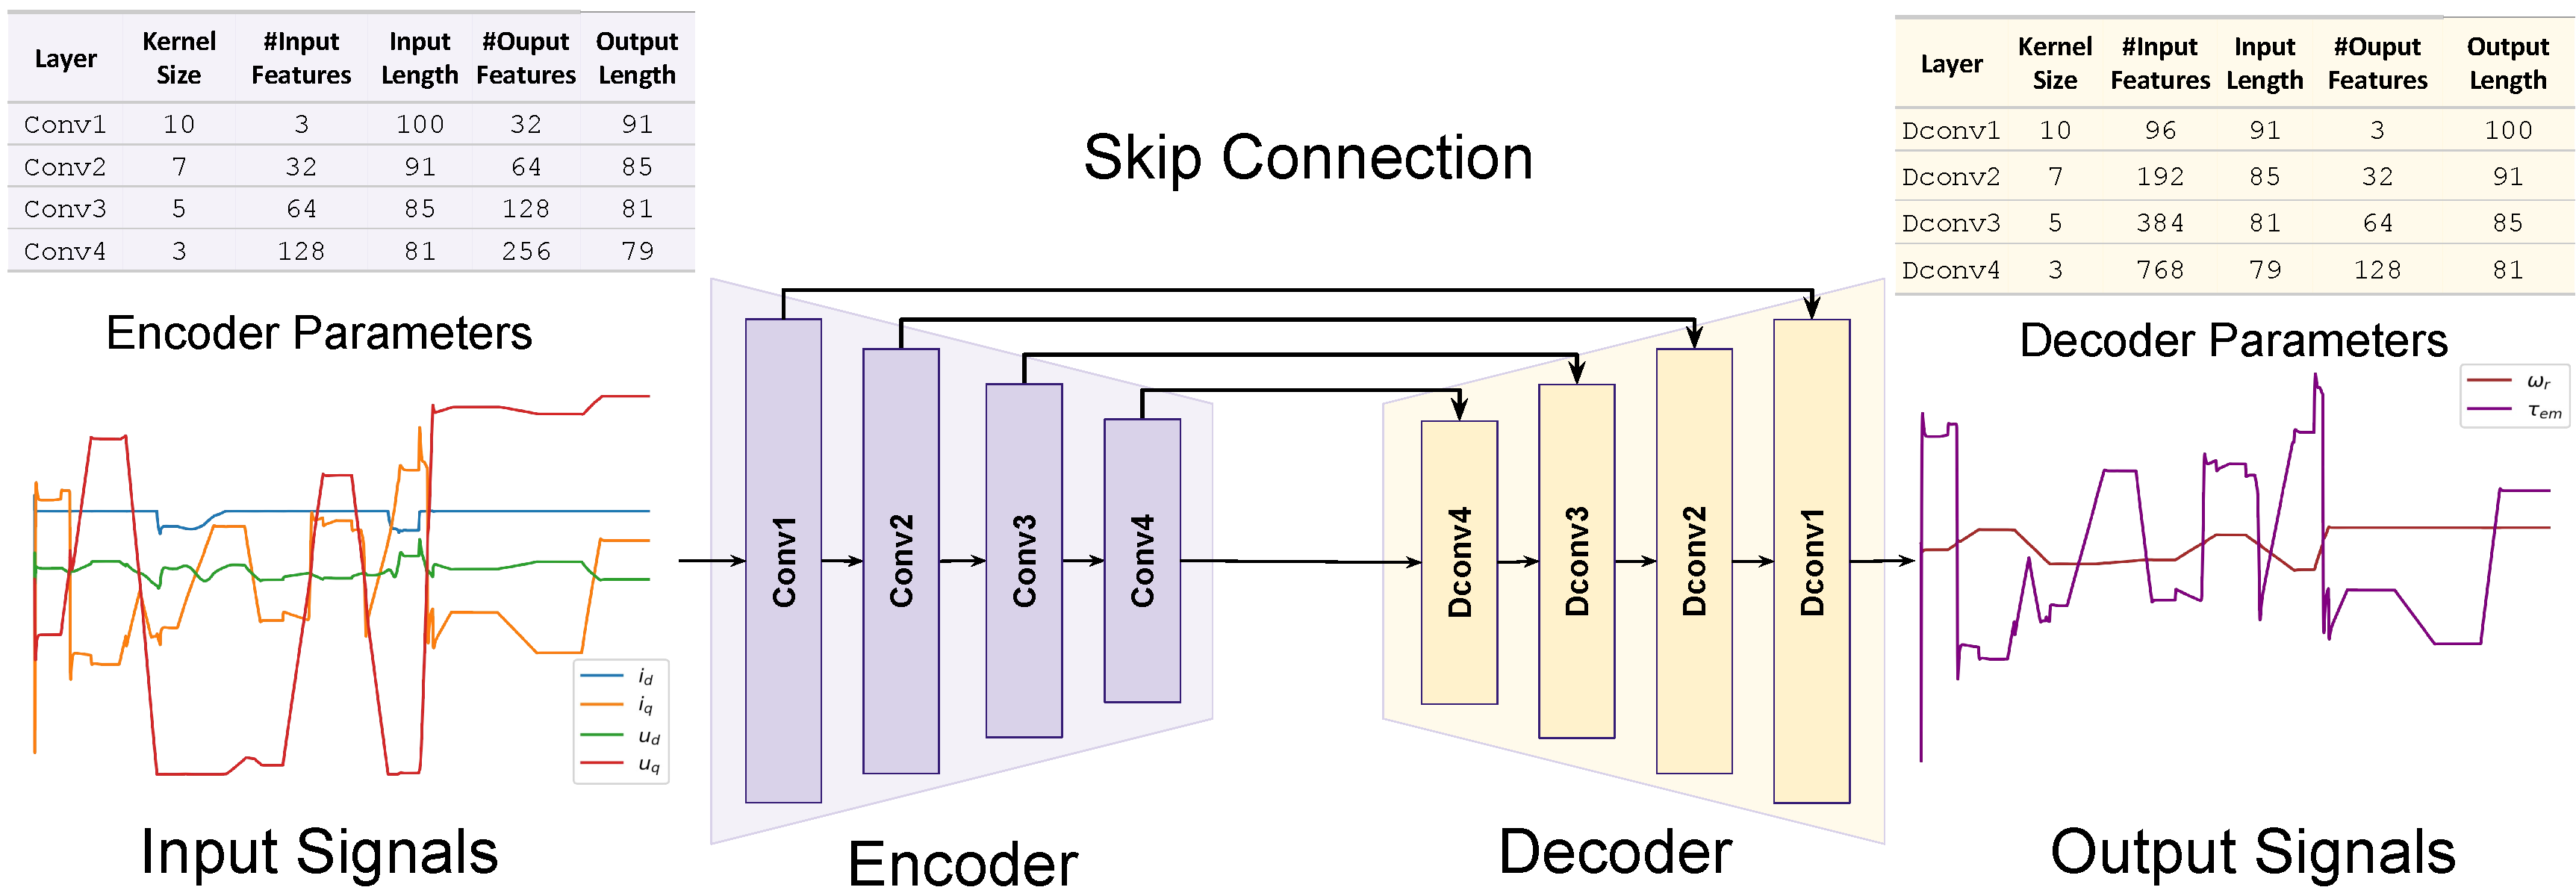
\includegraphics[scale=0.19]{images/ed_st_skip.pdf}
    \caption{Skip Connections}
    \label{fig:random}
    \vspace{-1em}
\end{figure}

\end{frame}

%---------------------------------------------------------
%Highlighting text
\begin{frame}
\frametitle{Encoder-Decoder with Recurrent Skip Connections (RNN)}

\begin{figure}[ht!]
    \centering
        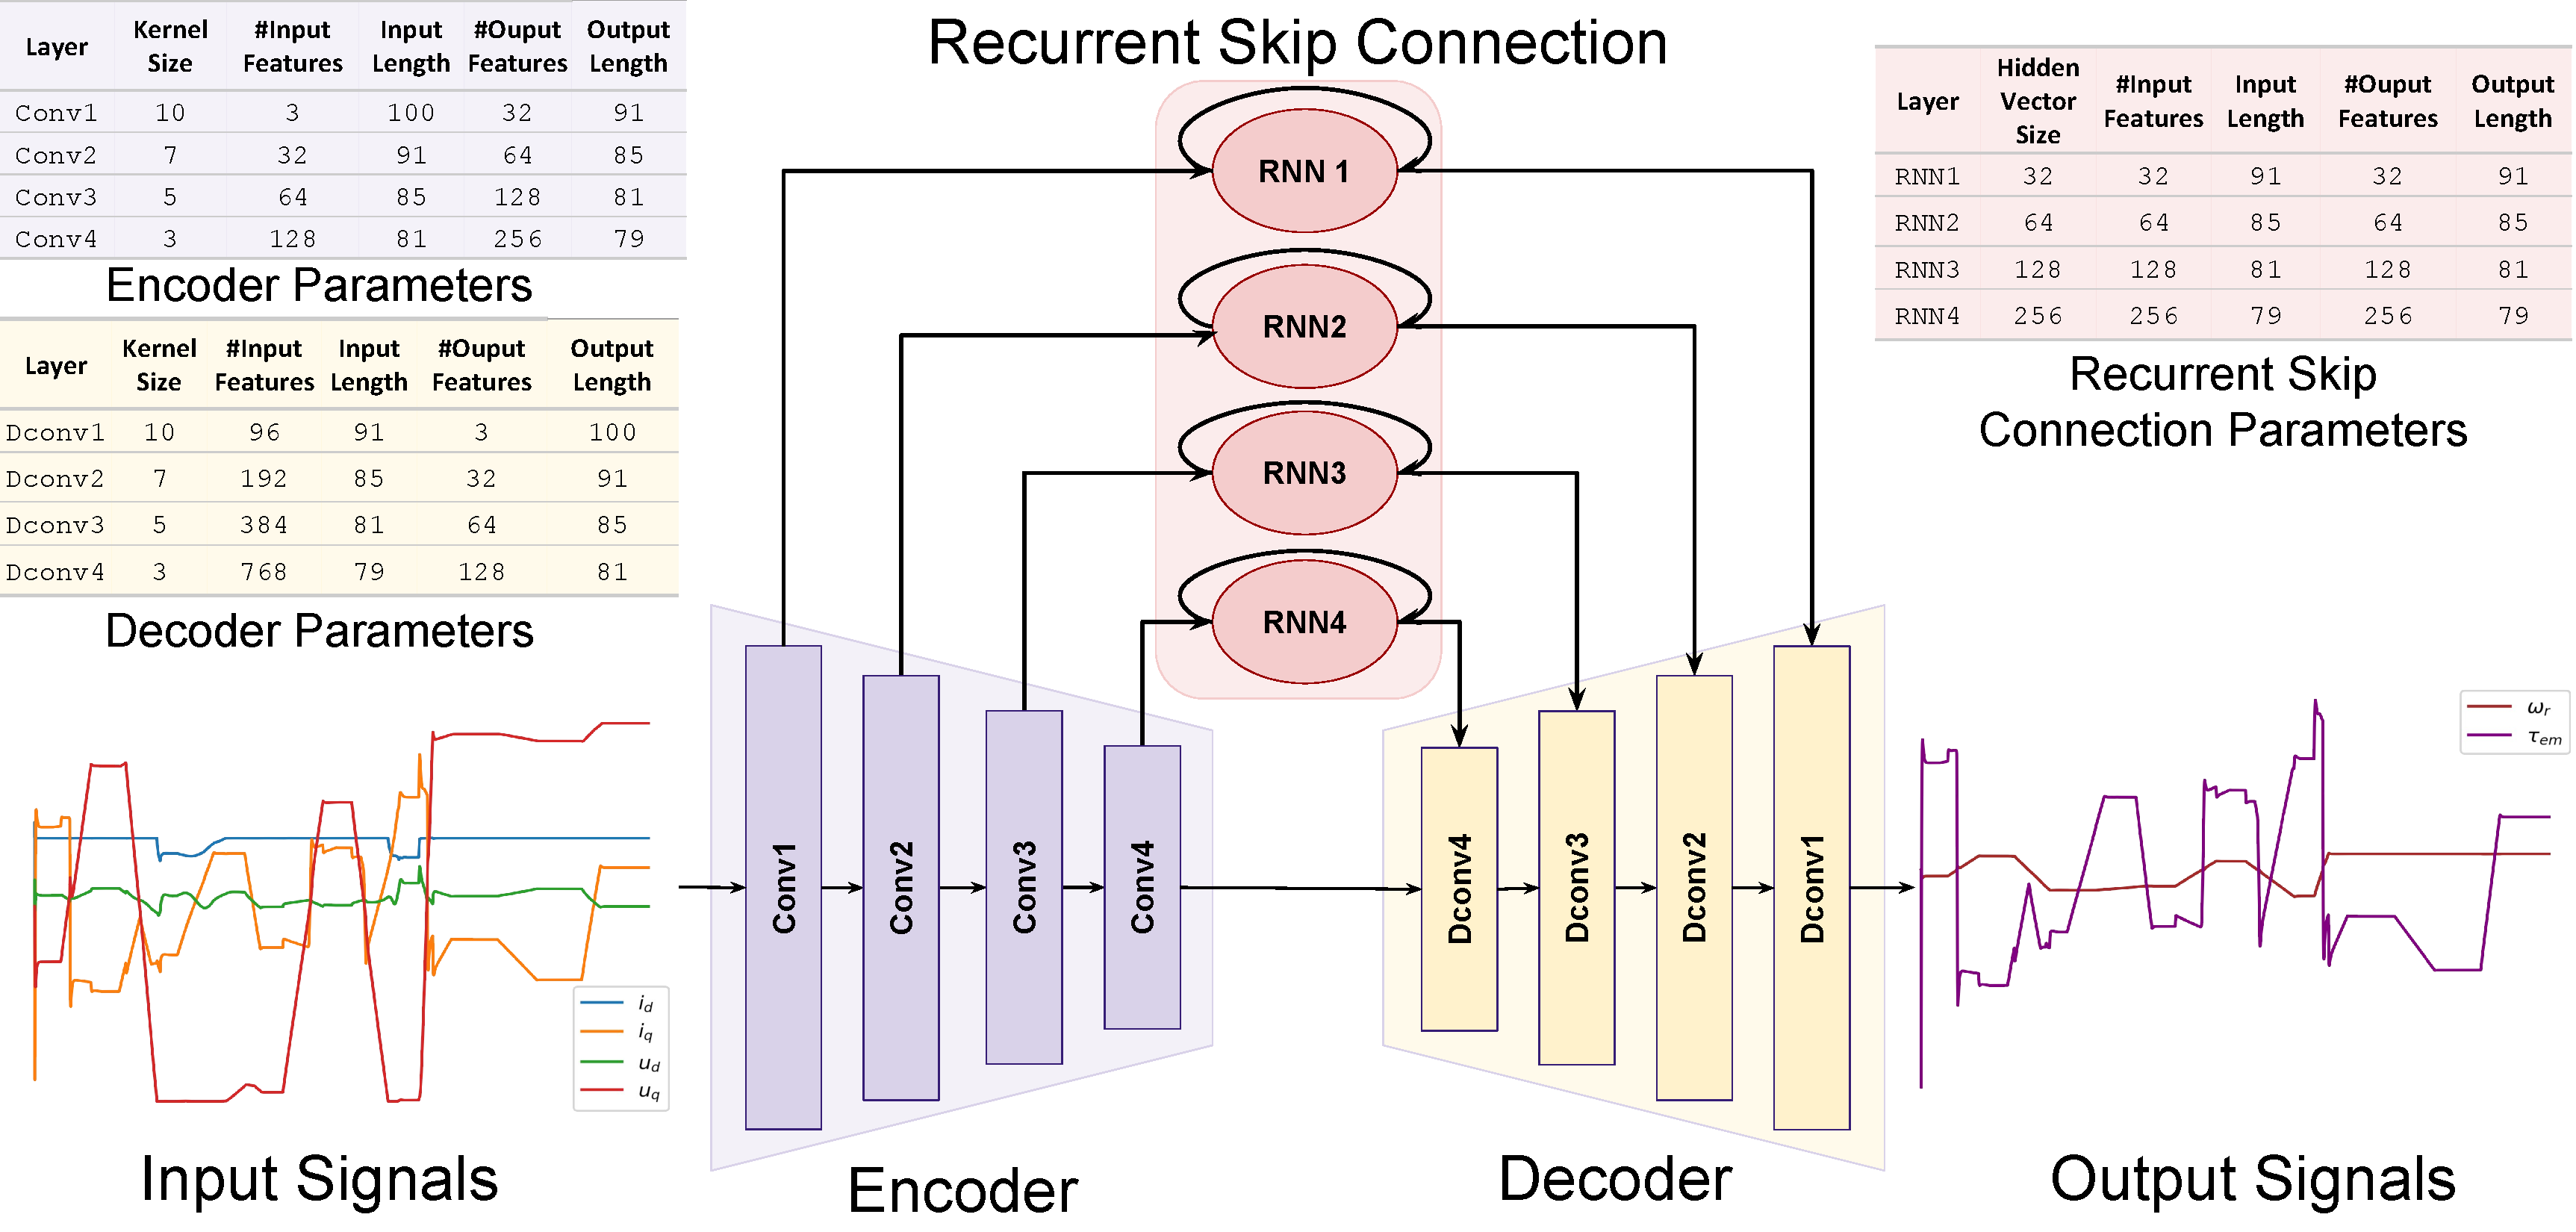
\includegraphics[scale=0.19]{images/ed_st_rnn.pdf}
    \caption{Recurrent Skip Connections}
    \label{fig:random}
    \vspace{-1em}
\end{figure}

\end{frame}

%---------------------------------------------------------
%Highlighting text
\begin{frame}
\frametitle{Encoder-Decoder with Bidirectional Recurrent Skip Connections (BiRNN)}

\begin{figure}[ht!]
    \centering
        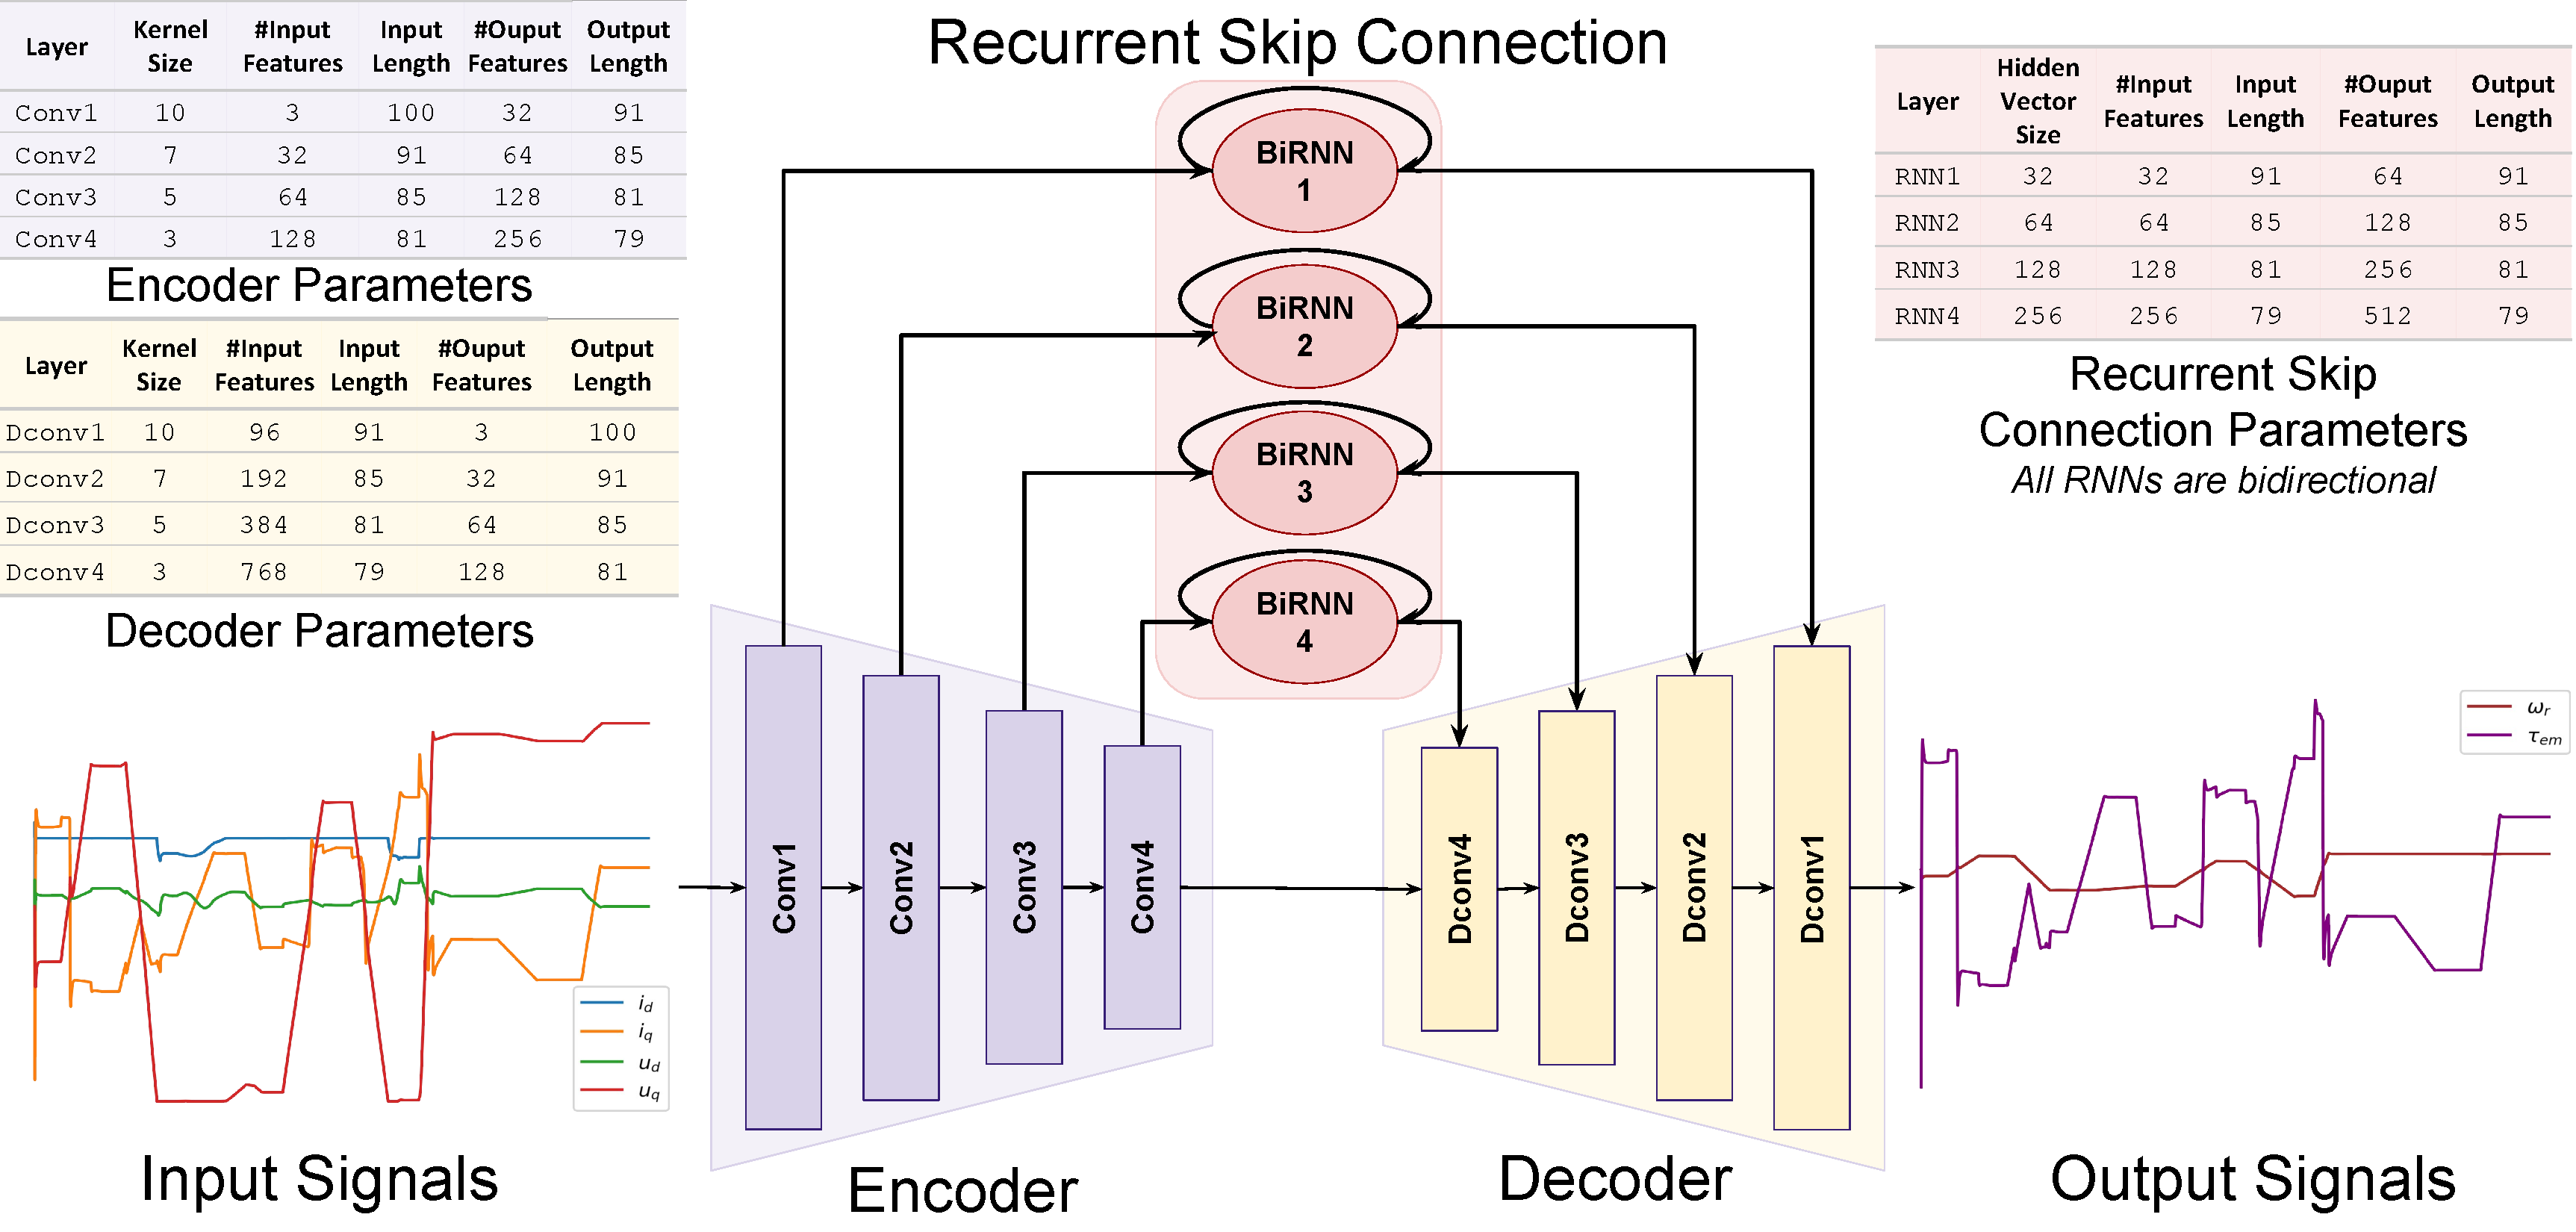
\includegraphics[scale=0.17]{images/ed_st_birnn.pdf}
    \caption{Bidirectional Recurrent Skip Connections}
    \label{fig:random}
    \vspace{-1em}
\end{figure}

\end{frame}

%---------------------------------------------------------
%Highlighting text
\begin{frame}
\frametitle{Encoder-Decoder with Bidirectional Diaganolized Recurrent Skip Connections (DiagBiRNN)}

\begin{figure}[ht!]
    \centering
        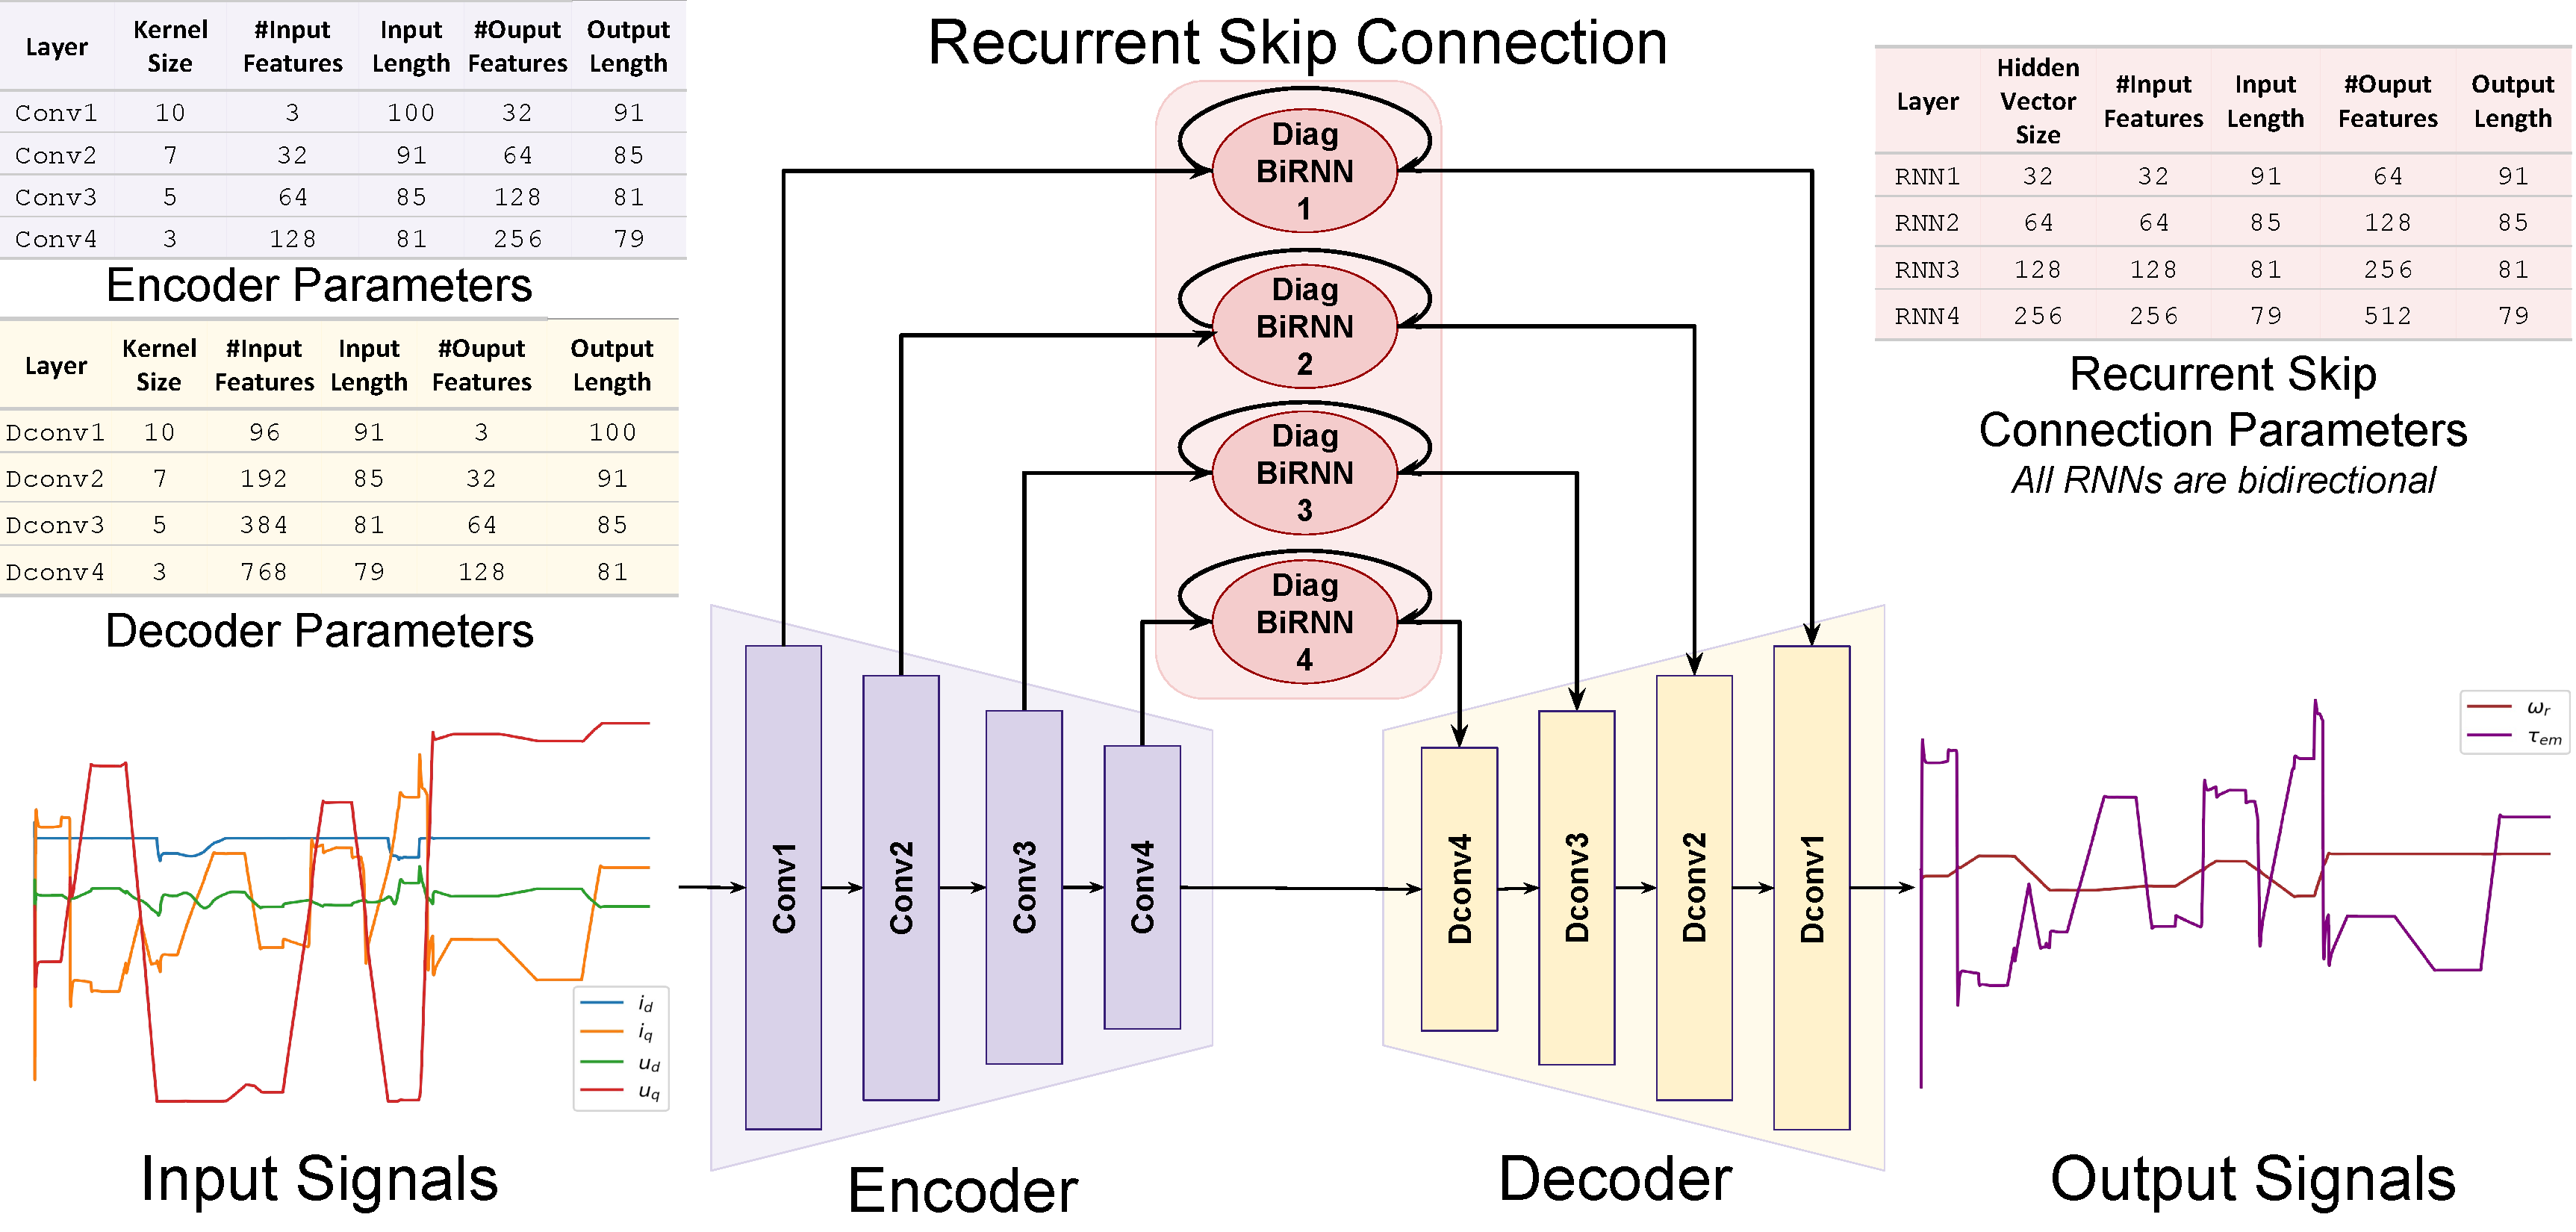
\includegraphics[scale=0.17]{images/encoder_decoder.pdf}
    \caption{Bidirectional Diaganolized Recurrent Skip Connections}
    \label{fig:random}
    \vspace{-1em}
\end{figure}

\end{frame}
%---------------------------------------------------------


%---------------------------------------------------------
%Highlighting text
\begin{frame}
\frametitle{Machine Learning Metrics}
Analyze neural network performance using ML metrics.

\begin{align*}
    \text{MAE}(y, \hat{y}) = \frac{1}{T}\sum^{T}_{t=1}|y_t - \hat{y}_t|
\end{align*}

\begin{align*}
    \text{SMAPE}(y, \hat{y}) = \frac{100}{T} \sum_{t=1}^T \frac{|\hat{y}_t-y_t|}{|\hat{y}_t|+|y_t|}
\end{align*}

\begin{align*}
   R^2(y,\hat{y}) = 1 - \frac{\sum^{T}_{t=1}(\hat{y}_t - \bar{y})^2}{\sum^{T}_{t=1}(y_t - \bar{y})^2}
\end{align*}
where $y_t$ is ground truth, $\hat{y}_t$ is predicted output at time $t$, and $T$ is total experiment duration. $\bar{y}$ is mean of ground truth $y$.

\end{frame}
%---------------------------------------------------------

%---------------------------------------------------------
%Highlighting text
\begin{frame}
\frametitle{Performance Metrics}
Electrical engineering (EE) performance metrics widely used in industrial settings.
\begin{itemize}
   \item \textbf{2\% response time ($t_{2\%}$)}
   \item \textbf{95\% response time ($t_{95\%}$)}
   \item \textbf{Overshoot ($D\%$)}
   \item \textbf{Steady-state error ($E_{ss}$)}
   \item \textbf{Following error ($E_{fol}$)}
   \item \textbf{Maximum acceleration torque (for speed ramp only) ($\Delta \tau_{max}$)}
   \item \textbf{Speed drop (for torque ramp only) ($SD$)}
\end{itemize}

\end{frame}
%---------------------------------------------------------


\section{Experiments}

%---------------------------------------------------------
%Highlighting text
\begin{frame}
\frametitle{Training and Validation Dataset Generation}
\begin{itemize}
    \item \textbf{100} simulated speed and torque trajectories.
    \item State-space model to simulate.
    \item Different speed and torque ramps from exponential distribution.
    \item \textbf{4kW} induction motor at \textbf{4kHz}.
    \item \textbf{150 minutes} of training and \textbf{30 minutes} of validation.
\end{itemize}

\end{frame}
%---------------------------------------------------------

%---------------------------------------------------------
%Highlighting text
\begin{frame}
\frametitle{Training and Validation Dataset Generation}

\begin{figure}[ht!]
    \centering
        \stackunder[6pt]{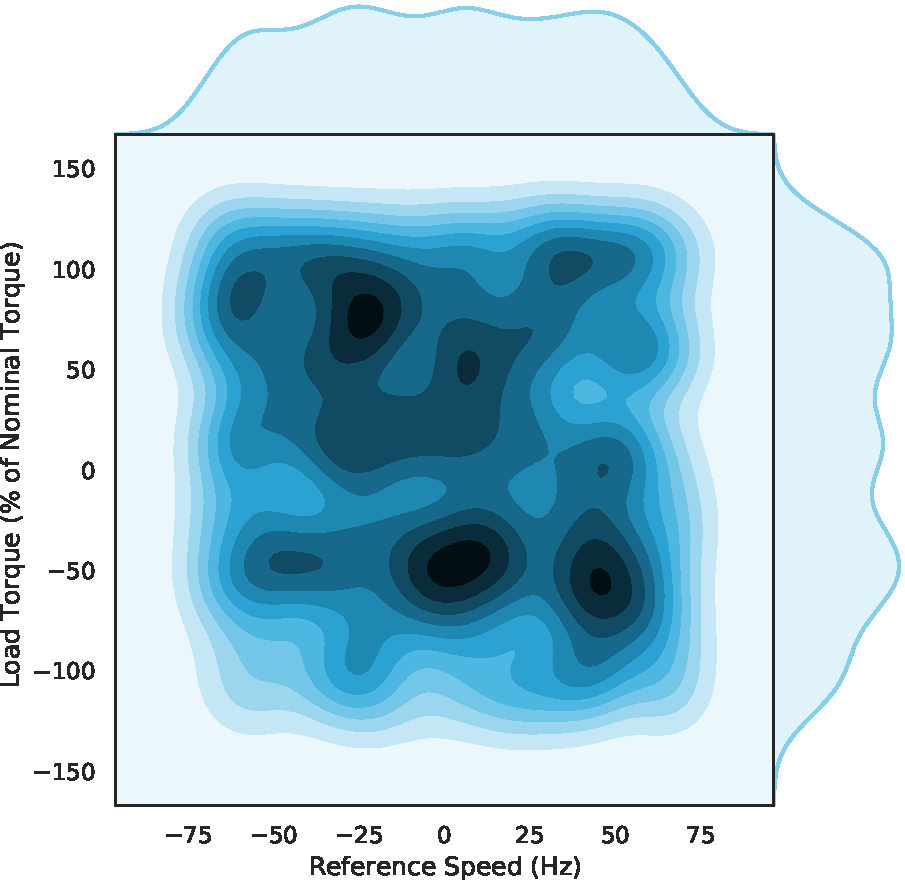
\includegraphics[scale=0.27]{images/training_zone.pdf}}{(a) Training zone}
        \stackunder[6pt]{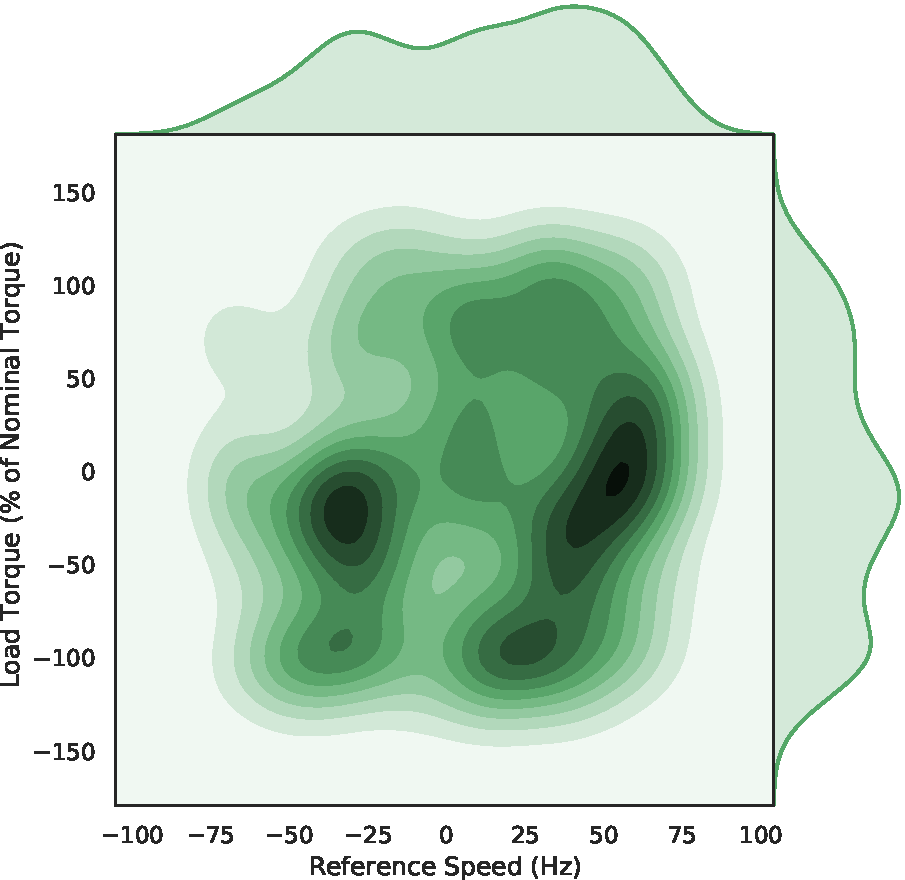
\includegraphics[scale=0.27]{images/validation_zone.pdf}}{(b) Validation zone}
    \caption{Density plots of torque vs speed plans showing training and validation separation.}
    \label{fig:zones}
    \vspace{-1em}
\end{figure}

\end{frame}
%---------------------------------------------------------

%---------------------------------------------------------
%Highlighting text
\begin{frame}
\frametitle{Ramps Distribution Matters}
\begin{figure}[ht!]
    \centering
    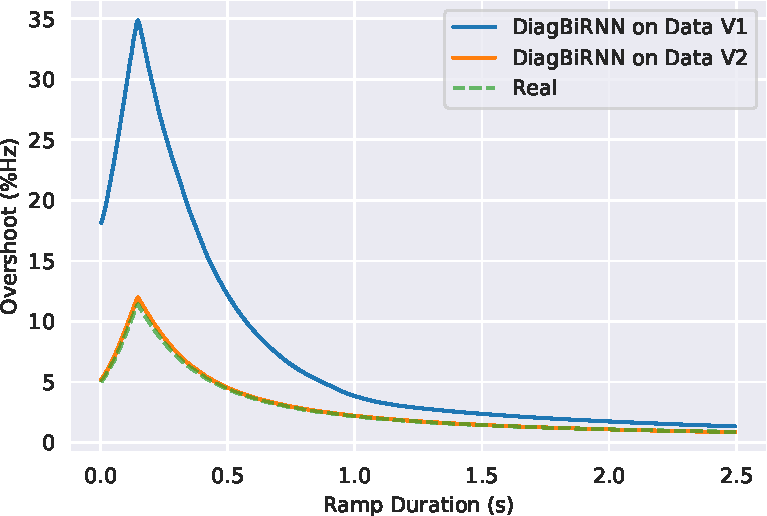
\includegraphics[scale=0.5]{images/goodbad.pdf}
    \caption{Overshoot vs. ramp. Bias in \textbf{Data V1} due to normal distribution. \textbf{Data V2} from exponential distribution.}
    \label{fig:goodbad}
    \vspace{-1em}
\end{figure}

\end{frame}
%---------------------------------------------------------


%---------------------------------------------------------
%Highlighting text
\begin{frame}
\frametitle{Test Dataset Generation}

Bench-marking NN methods using EE performance metrics.
\begin{itemize}
    \item \textbf{Dynamic-Speed1}: 0 to 50Hz in 1s at no load.
    \item \textbf{Dynamic-Speed2}: 50 to -50Hz in 1s at 50\% of nominal load.
    \item \textbf{Dynamic-Torque}: Load from 0 to 100\% of nominal in 4ms at 25Hz.
    \item \textbf{Quasi-Static1}: No load, 70 to -70Hz in 50s.
    \item \textbf{Quasi-Static2}: 50\% nominal load, 70 to -70Hz in 50s.
\end{itemize}
\end{frame}
%---------------------------------------------------------


%---------------------------------------------------------
%Highlighting text
\begin{frame}
\frametitle{Experimental Setup}
\begin{itemize}
    \item Ubuntu 18.04 OS, V100 GPU, and PyTorch.
    \item \textbf{Simulink} for state-space model.
    \item \textbf{100} time steps is the input size for all networks.
    \item Learning rate is \textbf{0.1} for standard and \textbf{0.001} for encoder-decoder.
    \item Total variation weighted mean square loss $\mathcal{L}_{\tiny{\text{TV-MSE}}}$.
\end{itemize}

\end{frame}
%---------------------------------------------------------




\section{Results and Conclusion}

%---------------------------------------------------------
%Highlighting text
\begin{frame}
\frametitle{Machine Learning Metrics Aggregated}
\begin{table}
    \centering
    \begin{tabular}{c c c c c}
        \toprule
          \multirow{2}{*}{\textbf{Model}} & \multicolumn{2}{c}{\textbf{Speed (\boldmath{$\omega_r$})}} & \multicolumn{2}{c}{\textbf{Torque (\boldmath{$\tau_{em}$})}} \\
          \cmidrule{2-5}
          &   \textbf{MAE} & \textbf{SMAPE} &  \textbf{MAE} & \textbf{SMAPE} \\
         \midrule
         \textbf{FCN}     & 0.79     & 21.77\%                   & 0.57    & 48.66\%   \\
         \textbf{LSTM}    & 0.11     & 18.76\%                   & 0.21    & 43.01\%   \\
         \textbf{CNN}     & 0.06     & 19.14\%                   & 0.09    & 38.91\%   \\
         \midrule
        \multicolumn{5}{c}{\textbf{\boldmath{$R^2$} is 0.99 for all the networks for both quantities.}} \\
         \bottomrule
    \end{tabular}
    \caption{ML metrics for the predictions done on benchmark set using standard models.}
\end{table}

\end{frame}
%---------------------------------------------------------


%---------------------------------------------------------
%Highlighting text
\begin{frame}
\frametitle{Machine Learning Metrics Aggregated}
\begin{table}
    \centering
    \begin{tabular}{c c c c c}
        \toprule
          \multirow{2}{*}{\textbf{Model}} & \multicolumn{2}{c}{\textbf{Speed (\boldmath{$\omega_r$})}} & \multicolumn{2}{c}{\textbf{Torque (\boldmath{$\tau_{em}$})}} \\
          \cmidrule{2-5}
          &   \textbf{MAE} & \textbf{SMAPE} &  \textbf{MAE} & \textbf{SMAPE} \\
         \midrule
         \textbf{Vanilla} & 0.05     & 18.94\%                     & 0.10    & 39.91\%   \\
         \textbf{Skip}    & 0.08     & 19.08\%                     & 0.12    & 43.23\%   \\
         \textbf{RNN}     & 0.06     & 19.31\%                     & 0.08    & 41.81\%   \\
         \textbf{BiRNN}   & 0.05     & \textbf{18.67\%}            & 0.09    & 42.82\%   \\
         \textbf{DiagBiRNN} & \textbf{0.03} & 18.76\%  & \textbf{0.04} & \textbf{38.46\%}  \\
         \midrule
        \multicolumn{5}{c}{\textbf{\boldmath{$R^2$} is 0.99 for all the networks for both quantities.}} \\
         \bottomrule
    \end{tabular}
    \caption{ML metrics for the predictions done on benchmark set using the encoder-decoder variants.}
\end{table}

\end{frame}
%---------------------------------------------------------


%---------------------------------------------------------
%Highlighting text
\begin{frame}
\frametitle{Performance Metrics on Dynamic Benchmarks}

\begin{table}[ht!]
    \centering
    \begin{tabular}{c c c c c c c}
        \toprule
          \textbf{Model} &   \shortstack{\boldmath{$t_{2\%}$} \\ (ms)} & \shortstack{\boldmath{$t_{95\%}$} \\ (ms)} & \shortstack{\boldmath{$E_{fol}$} \\ (Hz)} & \shortstack{\boldmath{$D\%$} \\ (\%)} & \shortstack{\boldmath{$E_{ss}$} \\ (Hz)} & \shortstack{\boldmath{$\Delta \tau_{max}$} \\ ($\%\tau_{nom})$} \\
         \midrule

\textbf{Real} & \textbf{48} & \textbf{960} & \textbf{-0.02} & \textbf{2.16} & \textbf{0.00} & \textbf{32.69} \\
\midrule
\textbf{Vanilla} & \leavevmode\color{good}44 & \leavevmode\color{good}968 & \leavevmode\color{good}-0.08 & 2.62 & \leavevmode\color{good}0.02 & 32.37 \\
\textbf{Skip} & \leavevmode\color{good}\textbf{48} & \leavevmode\color{good}952 & 0.12 & \leavevmode\color{bad}3.04 & \leavevmode\color{good}\textbf{0.01} & 32.46 \\
\textbf{RNN} & \leavevmode\color{good}\textbf{48} & \leavevmode\color{good}952 & \leavevmode\color{good}-0.04 & \leavevmode\color{good}2.28 & \leavevmode\color{good}0.02 & \leavevmode\color{good}32.82 \\
\textbf{BiRNN} & \leavevmode\color{good}44 & 944 & \leavevmode\color{good}-0.11 & \leavevmode\color{good}2.29 & \leavevmode\color{good}\textbf{0.01} & \leavevmode\color{good}\textbf{32.67} \\
\textbf{DiagBiRNN} & \leavevmode\color{good}44 & \leavevmode\color{good}952 & \leavevmode\color{good}\textbf{-0.01} & \leavevmode\color{good}\textbf{2.21} & \leavevmode\color{good}0.03 & \leavevmode\color{good}\textbf{32.67} \\
         \bottomrule
    \end{tabular}
    \caption{EE performance metrics obtained by encoder-decoder networks on Dynamic-Speed1 benchmark.}
    \label{tab:dynamicspeed1}
    \vspace{-1em}
\end{table}


\end{frame}
%---------------------------------------------------------

%---------------------------------------------------------
%Highlighting text
\begin{frame}
\frametitle{Performance Metrics on Dynamic Benchmarks}

\begin{figure}
    \centering
    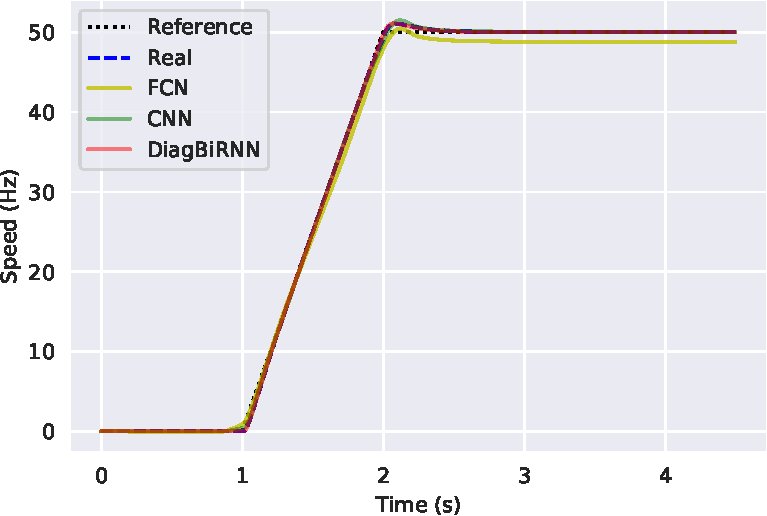
\includegraphics[scale=0.3]{images/bench1.pdf}
    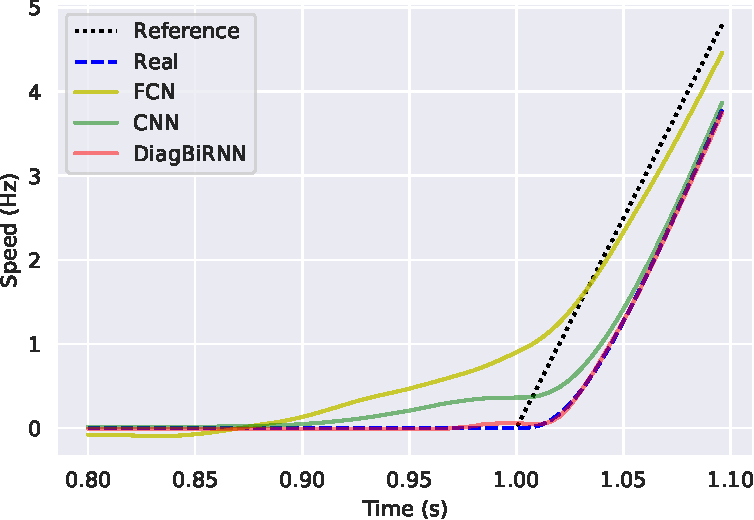
\includegraphics[scale=0.3]{images/bench1_1st.pdf} \\
    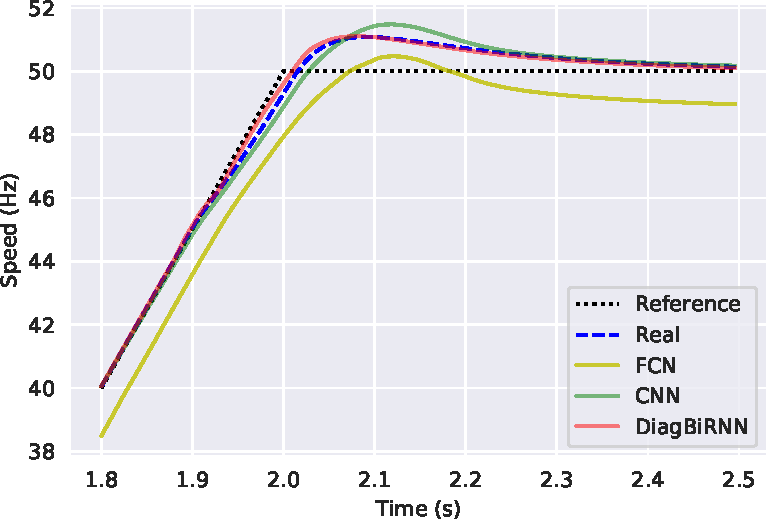
\includegraphics[scale=0.3]{images/bench1_3rd.pdf}
   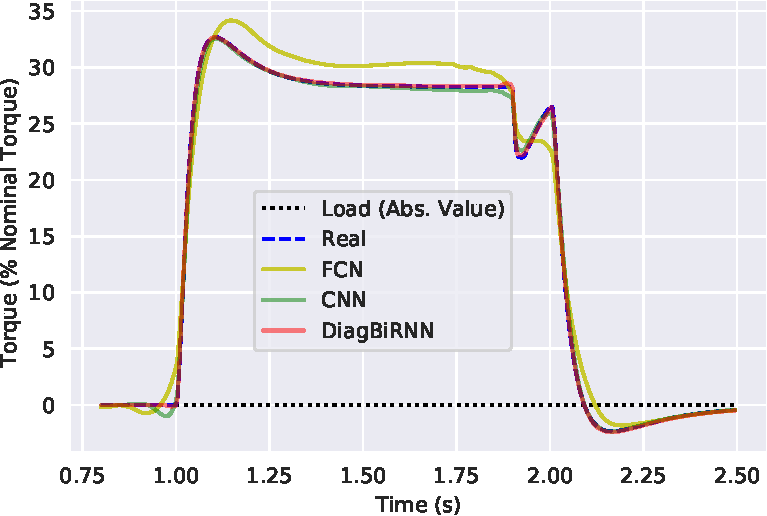
\includegraphics[scale=0.3]{images/bench1_torque.pdf} \\
    \label{fig:dynamicspeed1}
    \caption{Results on Dynamic-Speed1 benchmark.}
    \vspace{-1em}
\end{figure}

\end{frame}
%---------------------------------------------------------


% %Highlighting text
% \begin{frame}
% \frametitle{Performance Metrics on Dynamic Benchmarks}

% \begin{table}[ht!]
%     \centering
%     \begin{tabular}{c c c c c c c}
%         \toprule
%           \textbf{Model} &   \shortstack{\boldmath{$t_{2\%}$} \\ (ms)} & \shortstack{\boldmath{$t_{95\%}$} \\ (ms)} & \shortstack{\boldmath{$E_{fol}$} \\ (Hz)} & \shortstack{\boldmath{$D\%$} \\ (\%)} & \shortstack{\boldmath{$E_{ss}$} \\ (Hz)} & \shortstack{\boldmath{$\Delta \tau_{max}$} \\ ($\%\tau_{nom})$} \\
%          \midrule
% \textbf{Real} & \textbf{52} & \textbf{956} & \textbf{0.10} & \textbf{2.00} & \textbf{0.00} & \textbf{72.33} \\
% \midrule
% \textbf{Vanilla} & \leavevmode\color{good}44 & \leavevmode\color{good}\textbf{956} & 0.34 & \leavevmode\color{bad}3.55 & -0.11 & \leavevmode\color{good}72.29 \\
% \textbf{Skip} & \leavevmode\color{good}48 & \leavevmode\color{bad}1036 & \leavevmode\color{bad}0.45 & \leavevmode\color{bad}5.07 & -0.16 & \leavevmode\color{bad}71.28 \\
% \textbf{RNN} & \leavevmode\color{good}48 & 936 & 0.26 & \leavevmode\color{bad}3.89 & \leavevmode\color{good}\textbf{-0.06} & \leavevmode\color{good}72.25 \\
% \textbf{BiRNN} & \leavevmode\color{good}48 & 940 & 0.02 & \leavevmode\color{bad}3.28 & -0.13 & \leavevmode\color{good}72.45 \\
% \textbf{DiagBiRNN} & \leavevmode\color{good}\textbf{52} & \leavevmode\color{good}948 & \leavevmode\color{good}0.15 & \leavevmode\color{good}\textbf{2.39} & -0.12 & \leavevmode\color{good}72.15 \\
%          \bottomrule
%     \end{tabular}
%     \caption{EE performance metrics obtained by encoder-decoder networks on Dynamic-Speed2 benchmark.}
%     \label{tab:dynamicspeed1}
%     \vspace{-1em}
% \end{table}


% \end{frame}
%---------------------------------------------------------

%Highlighting text
\begin{frame}
\frametitle{Performance Metrics on Dynamic Benchmarks}

\begin{table}[ht!]
    \centering
    \begin{tabular}{c c c c c}
        \toprule
          \textbf{Model}   & \shortstack{\boldmath{$t_{95\%}$} \\ (ms)} & \shortstack{\boldmath{$D\%$} \\ (\%)} & \shortstack{\boldmath{$E_{ss}$} \\ ($\%\tau_{nom})$}  & \shortstack{\boldmath{$SD$} \\ (Hz)} \\
         \midrule
\textbf{Real} & \textbf{244}  & \textbf{15.96} & \textbf{0.00} & \textbf{4.39} \\
\midrule
\textbf{Vanilla}  & \leavevmode\color{good}\textbf{244}  & \leavevmode\color{bad}15.46 & \leavevmode\color{good}0.04 & \leavevmode\color{bad}3.88 \\
\textbf{Skip}  & \leavevmode\color{good}\textbf{244}  & \leavevmode\color{good}15.90 & \leavevmode\color{good}-0.02 & \leavevmode\color{good}\textbf{4.43} \\
\textbf{RNN}  & \leavevmode\color{good}\textbf{244}  & \leavevmode\color{good}15.87 & \leavevmode\color{good}\textbf{0.00} & \leavevmode\color{bad}4.03 \\
\textbf{BiRNN}  & \leavevmode\color{good}\textbf{244}  & \leavevmode\color{good}16.01 & \leavevmode\color{good}0.01 & 4.23 \\
\textbf{DiagBiRNN}  & \leavevmode\color{good}\textbf{244}  & \leavevmode\color{good}15.91 & \leavevmode\color{good}-0.02 & \leavevmode\color{good}4.31 \\
         \bottomrule
    \end{tabular}
    \caption{EE performance metrics obtained by different models on Dynamic-Torque benchmark.}
    \label{tab:dynamictorque}
    \vspace{-1em}
\end{table}


\end{frame}
%---------------------------------------------------------

%---------------------------------------------------------
%Highlighting text
\begin{frame}
\frametitle{Performance Metrics on Dynamic Benchmarks}

\begin{figure}
   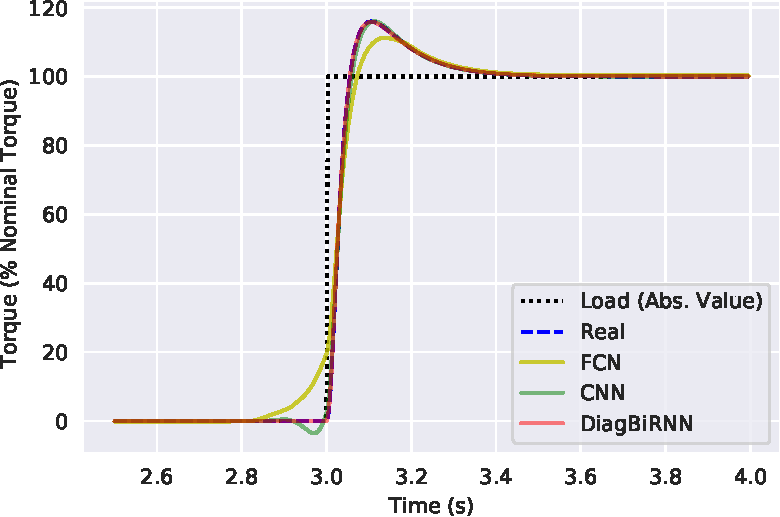
\includegraphics[scale=0.3]{images/bench4.pdf}
    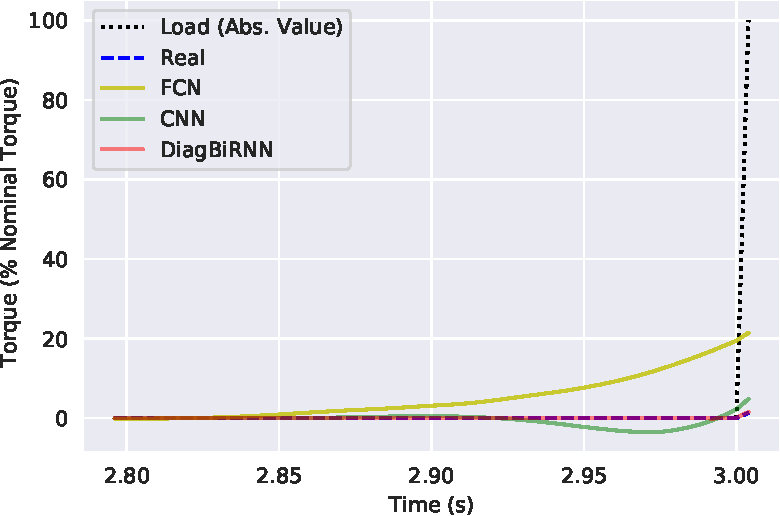
\includegraphics[scale=0.3]{images/bench4_1st.pdf} \\
    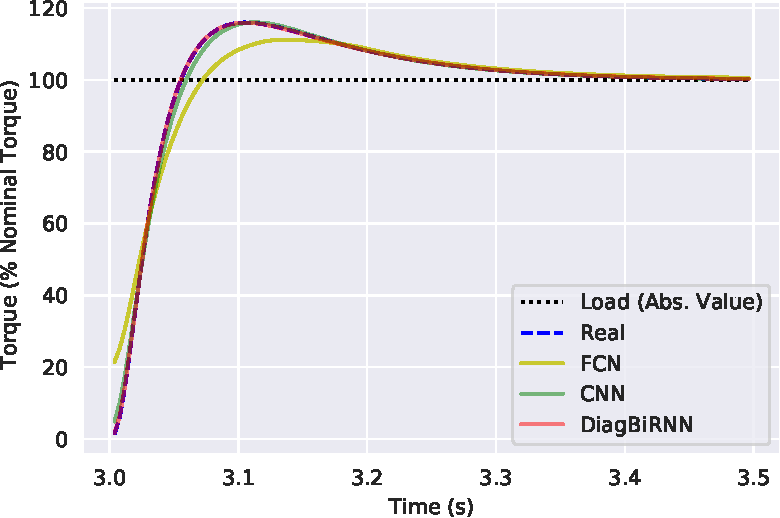
\includegraphics[scale=0.3]{images/bench4_3rd.pdf}
    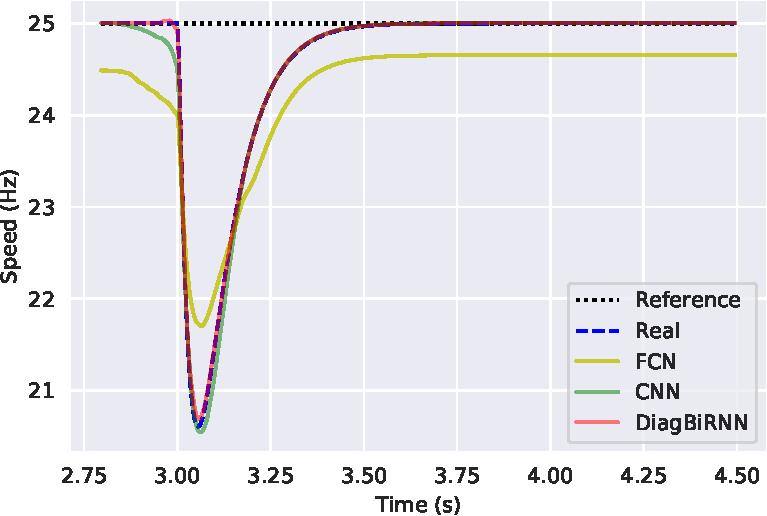
\includegraphics[scale=0.3]{images/bench4_speed.pdf}\\
    \caption{Results on Dynamic-Torque benchmark.}
    \label{fig:dynamictorque}
\end{figure}

\end{frame}
%---------------------------------------------------------

%---------------------------------------------------------
%Highlighting text
\begin{frame}
\frametitle{Performance Metrics on Static Benchmarks}


\begin{table}[ht!]
    \centering
    \begin{tabular}{c c c c c c c c}
        \toprule
          \textbf{FCN} & \textbf{LSTM} & \textbf{CNN} & \textbf{Vanilla} & \textbf{Skip} & \textbf{RNN} & \textbf{BiRNN} & \textbf{DiagBiRNN} \\
         \midrule
          3.66 & 0.992 & 0.261 & 0.178 & 0.549 & 0.341 & 0.236 & \textbf{0.198}\\
          \bottomrule
        \vspace{-1em}
        \end{tabular}
    \caption{Max absolute error (Hz) for Quasi-Static1 benchmark.}
    \label{tab:qs}
    \vspace{-1em}
\end{table}

\begin{figure}[ht!]
    \centering
    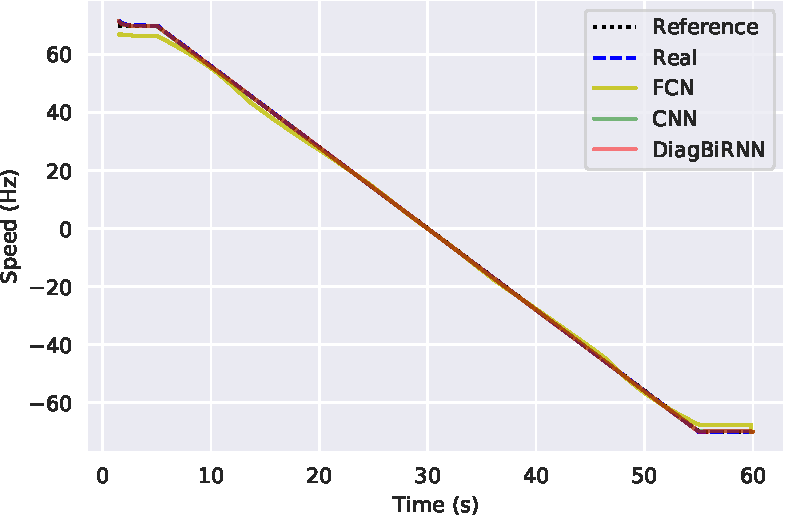
\includegraphics[scale=0.3]{images/bench5.pdf}
    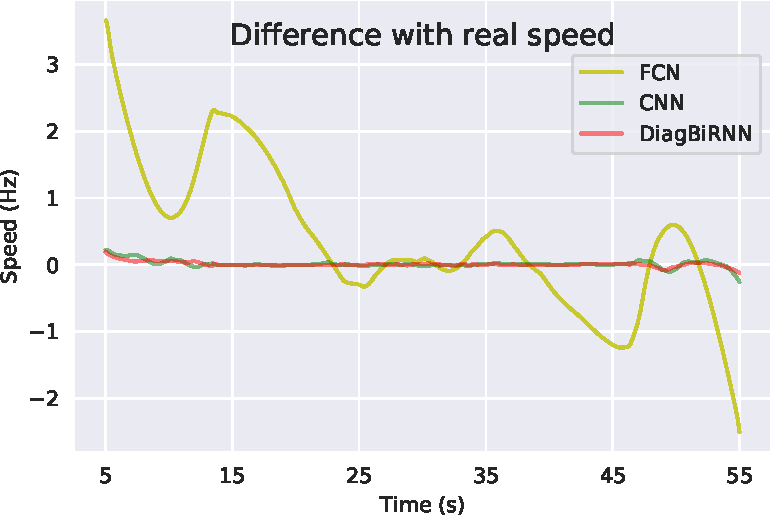
\includegraphics[scale=0.3]{images/bench5_dif.pdf}
    \vspace{-1em}
    \caption{Results on Quasi-Static1 benchmark.}
    \label{fig:static1}
    \vspace{-1em}
\end{figure}



\end{frame}
%---------------------------------------------------------

\begin{frame}
\frametitle{Conclusion}
    \begin{itemize}
        \item NNs for speed-torque estimation are not trivial.
        \item Special care in dataset generation and training procedure.
        \item ML metrics gives false sense performance gain.
        \item EE performance metrics are best suited for this kind of problems.
    \end{itemize}
\end{frame}

\begin{frame}{}
  \centering \Large
  \emph{Thanks!} \\
  \emph{Contact: sagar.verma@se.com}

    \begin{figure}[ht!]
    \centering
    
\includegraphics[scale=0.5]{images/qr.png}
    \vspace{-1em}
    \caption{Project page, code, and dataset.}
    \label{fig:static2}

\end{figure}

\end{frame}


\end{document}
